\chapter{Network monitoring with segment routing}
\label{chapter:scmon}


\section*{Introduction}

Monitoring is a crucial task for network operations. It is needed to ensure that all resources operate correctly (e.g., no
failures) and their configuration meets operator’s expectations (no congestion, required quality of service, etc.). Effective
monitoring is also fundamental for management tasks like traffic engineering, maintenance and troubleshooting.

\begin{figure}
\begin{center}
\includegraphics[width=.85\columnwidth]{figures/ovh-eu.pdf}
\end{center}
\caption{European backbone of \textsf{OVH}. In contrast to prior techniques, our algorithm can monitor health and performance of single
links in bundles (e.g., between \textsf{LONDON} and \textsf{ROUBAIX}).}
\label{fig:ovh}
\end{figure}


Unfortunately, even basic monitoring tasks, like checking for hardware malfunctions, are practically hard, due to the
complexity of current networks. Prominently, multi-path routing is widely used, both to spread the load on multiple paths
and to aggregate parallel links in bundles.
Figure \ref{fig:ovh} shows an overview of the European backbone of a big cloud provider,
\textsf{OVH}. It highlights that parallel links are used at the same time between many pairs of routers. While enabling better
performance and robustness, multi-path routing also poses significant obstacles to monitoring. For instance, assessing
the exact path and performance of each packet becomes complex [2], [20] since such a path depends on (vendor-specific) hash functions used by routers for load-balancing.

As a consequence, not only naive approaches (e.g., based on ping or traceroute) are not sufficient, but also 
state-of-the-art monitoring techniques tend to be ineffective.


On the one hand, protocol-based approaches use control-plane messages to infer possible failures. 
For example, link-state routing protocols (like OSPF or IS-IS) or specialized
ones (BFD [14]) rely on heartbeat-like mechanisms to check
bi-directional connectivity among pairs of adjacent nodes. This
approach only ensures detection of failures that affect control plane messages. 
However, it cannot be used to detect failures that only affect data-plane traffic like: 

\begin{enumerate}[i)]
\item corruption of an
optical link that leads to framing errors and packet losses;
\item malfunctioning of a router interface that considers the link still up but discards all the received packets;
\item failure of only one link among the parallel ones between two routers.
\end{enumerate}

On the other hand, probe-based techniques rely on sending
data-plane monitoring packets, i.e., probes, between fixed
vantage points in the network. Vantage points typically run
standard protocols (e.g., IPSLA [8]) to send probes and extract
measurements from them. Unfortunately, if the probes are sent
over paths used to forward regular traffic, many vantage points
may be needed to obtain high coverage, and links not used
by current paths (e.g., backup links) cannot be checked at
all. Otherwise, probes can be sent over tunnels (e.g., RSVP-TE [3] ones) to enforce specific paths, but this is not scalable.
Indeed, even for detecting single-link failures and pinpointing
their position, the number of needed tunnels tends to explode,
and so does the control-plane overhead (to signal tunnels) [7].

We propose a new technique that ensures full coverage of all network resources from a
single vantage point. It is based on sending data-plane probes over carefully-chosen cycles. This way, a single box can both
send and receive monitoring probes, avoiding the need for synchronizing and coordinating multiple vantage points, hence
minimizing infrastructural costs. By relying on data-plane measurements, we support both detection of hardware failures and resource overloading (e.g., link congestion).

% Segment routing generates conflicting objectives for the computation
% of cycles over which probes are sent. On the one hand, we would like to minimize the number of cycles, to reduce the
% monitoring overhead; hence, we should have cycles that are long and few in number. On the other hand, we need cycles
% to be enforced in practice, and long cycles may require too many segments even for the most powerful commercial routers
% (currently supporting less than 10 segments). To tackle those challenges, SCMon runs original algorithms
% that compute cycles on a monitoring topology, maintained by routers in addition to the one used for user traffic. The monitoring topology spans all network links, 
% and uses carefully computed weights that avoid (as much as possible) ECMP paths, i.e., multiple shortest paths between a pair of nodes.
% Note that existing routers have already been shown to well support two topologies and their (limited) overhead [17].
% SCMon supports detection and localization of any set of link failures/overloading. It infers single-link failures by keeping
% track of the cycles associated to probes sent and not received at the monitoring box. For multiple link failures, we have two
% cases. Some of them, e.g., affecting links in disjoint cycles, are detected directly from the set of lost probes (as single-link failures). 
% The others, e.g., affecting two links belonging to a single monitoring cycle, are reported by SCMon one at
% a time: This provides operators with a debugging interface (asking to correct one error before showing another one)
% similar to the one of a compiler for software programs. Similar considerations apply to node failures and link congestion.
% In developing SCMon, we make three main contributions.
% 
% Our approach to compute monitoring cycles consists of four steps.
% The first step computes IGP weights for the monitoring topology, in order to minimize ECMP paths.
% The second step models link bundles aggregated into a single IGP link. 
% The third step calculates a set of cycles covering the whole network and sharing the node from which probes are sent.
% The last step computes the SR segments to send probes over those cycles.


%In this section we will propose several algorithms and strategies to compute a cycle cover of the network
%using segment routing. We need however to impose some properties in the cycle cover in order to be able to use
%it for detecting single link failures in a network. Those properties as the following:

As usual, we start by defining the problems that we tackle in this chapter. To do that we need the two following definitions.
Throughout this chapter we assume that the network topology is symmetric.

\begin{definition}
Let $G$ be a symmetric network, $s \in V(G)$ and $k \in \mathbb{N}$. We denote by $\mathcal{C}^k_s$ the set of deterministic sr-cycles from $s$ to $s$ with segment cost at most $k$.
\end{definition}

\begin{definition}
Let $G$ be a symmetric network, $s \in V(G)$ and $k \in \mathbb{N}$. A \emph{$k$ sr-cycle cover} of a network $G$ 
with vantage point $s$ is a subset $C \subseteq \mathcal{C}^k_s$ of deterministic sr-cycles such
that for each edge $e \in E(G)$ there exists $\sr{c} \in C$ such that $e \in E(\sr{c})$.
\end{definition}

Below we define the two problems that we tackle in this chapter. Both of them seek to compute a cycle cover.
The first aims at minimizing the maximum segment cost of any sr-cycle in the cover while the second wants to minimize the number of cycles for a given segment cost limit.
% We will see that the first problem admits a polynomial time solution and that the second one is \NPhard.


\begin{problem}{Min segment cost cover}
\label{prob:min-seg-cover}
\textbf{Input:} A symmetric network $G$ and $s \in V(G)$.

\textbf{Output:} A sr-cycle cover $C$ of $G$ such that the maximum segment cost of any sr-cycle $\sr{c} \in C$ is minimum.
\end{problem}

\begin{problem}{Min sr-cycle cover}
\label{prob:min-cycle-cover}
\textbf{Input:} A symmetric network $G$, $s \in V(G)$ and $k \in \mathbb{N}$.

\textbf{Output:} A sr-cycle cover $C \subseteq \Csk$ of $G$ such that $|C|$ is minimum.
\end{problem}
% 
% \begin{proposition}
% Problem \ref{prob:min-cycle-cover} is \NPhard.
% \end{proposition}
% 
% \begin{proof}
% The problem of finding a minimum cardinaly cycle cover of a graph is \NPhard and by setting $k$
% large enough and setting IGP weights such that there is not ECMP any solution
% to Problem \ref{prob:min-cycle-cover} corresponds to a minimum cycle cover.
% \end{proof}
% 


\input{chapters/monitoring/min-seg-cover}

\section{The idea behind Column Generation}

% \todo{
% Structure: 1. Explain LP duality. 2. show that removing variables from primal = remove constraints from dual. 3. constraints is easier to check, with a partial solution
% of the primal we can map to the dual and check for constraints viaolation. if not violation optimal. maybe show concrete example before.
% }
% 
% 
% Strong duality \todo{ref} tell us that there exists another LP, called the dual, and that for any feasible solution $x$
% of the primal

We now describe how we used Column Generation (CG) \cite{desaulniers2006column} to overcome the model size problems faced when using the path model for
solving the traffic engineering problem with SR. CG is usually used to solve linear programs with a huge number of variables. The idea is to solve the problem for a subset
of the variables and then incrementally insert the missing variables, slowly growing the model. Each time that we add new variables, we solve the model again to check
for optimality. One could ask what
is the point of doing this since at some point we will have the whole set of variables, so why not just solve the full problem instead? However, we will carefully select the 
new variables that we introduce so that in general this framework will reach an optimal solution to the original \emph{problem without ever needing to consider all variables}.

To understand the impact of ignoring a variable and how we can prove optimality without considering all variables, we work out a small example. 
This will allow us to explain the main idea behind CG in a much more 
intuitive way by providing an example without overwhelming mathematical notations. Suppose that we have the following LP that we want to solve.

\begin{center}
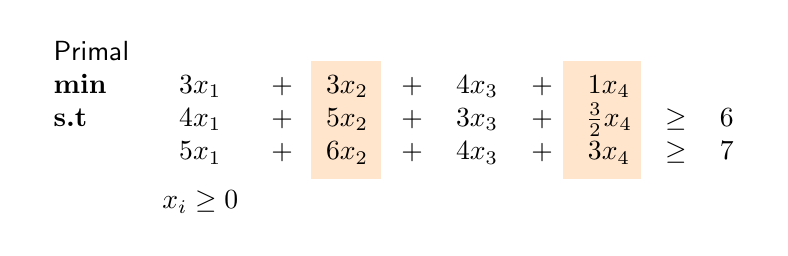
\begin{tikzpicture}
\def\x{0}
\def\y{0}
\fill[orange!20!white] (\x + 4 - 0.4, \y + 0 - 0.425) rectangle (\x + 4.9 - 0.4, \y + -1.5 - 0.425);
\fill[orange!20!white] (\x + 7.2 - 0.4, \y + 0 - 0.425) rectangle (\x + 8.1 - 0.3, \y + -1.5 - 0.425);
\node[anchor=north west] (primal) at (\x, \y) {
\begin{tabular}{lcccccccccc}
\textsf{Primal} & & & & & & & & & \\
$\displaystyle \mathbf{min}$ & $3 x_1$ & $+$ & $3 x_2$ & $+$ & $4 x_3$ & $+$ & $1 x_4$ & & \\
\textbf{s.t} & $4 x_1$ & $+$ & $5 x_2$ & $+$ & $3 x_3$ & $+$ & $\frac{3}{2} x_4$ & $\geq$ & $6$ \\
             & $5 x_1$ & $+$ & $6 x_2$ & $+$ & $4 x_3$ & $+$ & $3 x_4$ & $\geq$ & $7$ \\[0.2cm]
& $x_i \geq 0$ & & & & & & & &
\end{tabular}
};
\end{tikzpicture}
\end{center}

The dual of this problem can be obtained by following a systematic procedure. By doing so, we obtain the following linear program.
\begin{center}
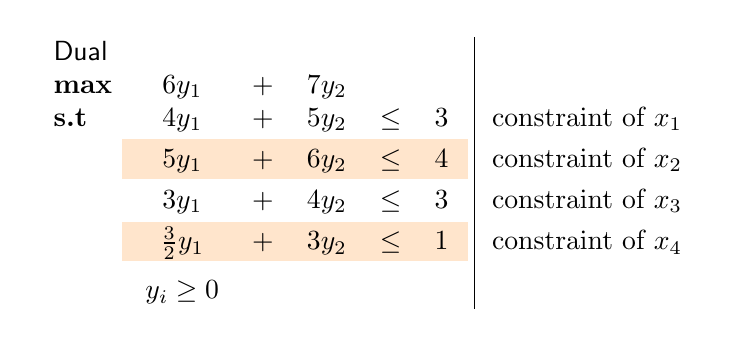
\begin{tikzpicture}
\def\x{0}
\def\y{0}
\fill[orange!20!white] (\x + 2 - 0.8, \y + -1 - 0.425) rectangle (\x + 5.6, \y + -1.5 - 0.425);
\fill[orange!20!white] (\x + 2 - 0.8, \y + -1.2 - 3 * 0.425) rectangle (\x + 5.6, \y + -1.7 - 3 * 0.425);
\node[anchor=north west] (dual) at (\x, \y) {
\begin{tabular}{lccccc | r}
\textsf{Dual} & & & & & \\
$\mathbf{max}$ & $6 y_1$ & $+$ & $7 y_2$ & &  \\
\textbf{s.t} & $4 y_1$ & $+$ & $5 y_2$ & $\leq$ & $3$ \quad & constraint of $x_1$ \\[0.1cm]
             & $5 y_1$ & $+$ & $6 y_2$ & $\leq$ & $4$ \quad  & constraint of $x_2$ \\[0.1cm]
             & $3 y_1$ & $+$ & $4 y_2$ & $\leq$ & $3$ \quad  & constraint of $x_3$ \\[0.1cm]
             & $\frac{3}{2} y_1$ & $+$ & $3 y_2$ & $\leq$ & $1$  \quad  & constraint of $x_4$ \\[0.2cm]
& $y_i \geq 0$ & & & &
\end{tabular}
};
\end{tikzpicture}
\end{center}

Each variable $x_i$ of the primal corresponds to a constraints of the dual. So, for instance, $x_2$ corresponds to constraint
$5 y_1 + 6 y_2 \geq 4$ and $x_4$ corresponds to the constraint $\frac{3}{2} y_1 + 3 y_2 \geq 1$ as highlighted in the models.

Because of this correspondence, when we ignore a variable on the primal, this translates in the dual to ignoring the corresponding constraint. 
For example, if we consider the restricted primal problem on variables $x_1$ and $x_3$ only (that we denote by $\textsf{Primal}(1, 3)$), 
and we take the dual, the dual will be the same as above but 
will only have the first and third constraints.

\begin{center}
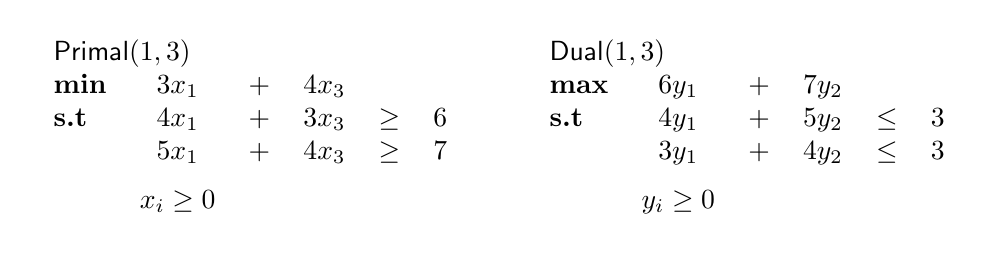
\begin{tikzpicture}
\def\x{0}
\def\y{0}
\node[anchor=north west] (primal) at (\x, \y) {
\begin{tabular}{lcccccccccc}
\multicolumn{11}{l}{$\textsf{Primal}(1, 3)$} \\
$\mathbf{min}$ & $3 x_1$  & $+$ & $4 x_3$ & & \\
\textbf{s.t} & $4 x_1$  & $+$ & $3 x_3$ & $\geq$ & $6$ \\
& $5 x_1$ & $+$ & $4 x_3$ & $\geq$ & $7$ \\[0.2cm]
& $x_i \geq 0$ & & & &
\end{tabular}
};

\def\x{6.3}
\def\y{0}
\node[anchor=north west] (dual) at (\x, \y) {
\begin{tabular}{lccccc}
\multicolumn{6}{l}{$\textsf{Dual}(1, 3)$} \\
$\mathbf{max}$ & $6 y_1$ & $+$ & $7 y_2$ & &  \\
\textbf{s.t} & $4 y_1$ & $+$ & $5 y_2$ & $\leq$ & $3$ \\
& $3 y_1$ & $+$ & $4 y_2$ & $\leq$ & $3$ \\[0.2cm]
& $y_i \geq 0$ & & & &
\end{tabular}
};
\end{tikzpicture}
\end{center}

Suppose that we solve the restricted primal we obtain the optimal solution $x^* = (1.5, 0)$. By duality, we also obtain 
an optimal solution $y^*$ of the restricted dual. In this case $y^* = (0.75, 0)$. From here, we want to be able to decide whether $x^*$ is actually optimal
for the original primal problem and, if not, what new variable $x_2$ or $x_4$ should we consider to improve the solution. By strong
duality, we know that $x^*$ is optimal for \textsf{Primal} if and only if $y^*$ is optimal for \textsf{Dual}. Since the only 
difference between \textsf{Dual} and $\textsf{Dual}(1, 3)$ is that we removed two constraints from \textsf{Dual}, $y^*$
contains values for \emph{all} variables of the dual. Therefore,
to check the optimality of $y^*$ for \textsf{Dual}, we can plug its values into the missing constraints to check whether $y^*$ satisfies them. 
If $y^*$ happens to satisfy all of them, then it must be optimal for the unrestricted dual and by consequence, $x^*$ is optimal for the
unrestricted original primal.
In this example, for the constraint corresponding to $x_2$ we have
\begin{align*}
5 y_1 + 6 y_2 = 5 \cdot 0.75 + 6 \cdot 0 = 3.75 > 3
\end{align*}
and for the constraint corresponding to $x_4$ we have
\begin{align*}
2 y_1 + 6 y_2 = 2 \cdot 0.75 + 6 \cdot 0 = 1.5 > 1. \\
\end{align*}
Both of them are violated so we cannot conclude that $y^*$ is optimal for \textsf{Dual}. So we chose one of $x_2, x_4$ to be added to the model.
For the sake of example, we choose $x_2$ obtaining (we highlighted in green the newly added column):

\begin{center}
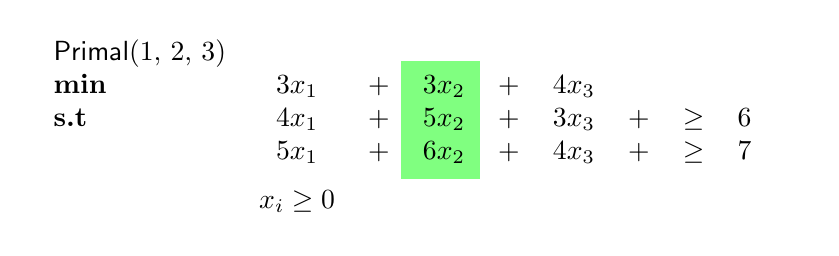
\begin{tikzpicture}
\def\x{0}
\def\y{0}
\fill[green!50!white] (\x + 4 + 1.15 - 0.4, \y + 0 - 0.425) rectangle (\x + 5 + 1.15 - 0.4, \y + -1.5 - 0.425);
\node[anchor=north west] (dual) at (\x, \y) {
\begin{tabular}{lcccccccccc}
\textsf{Primal}(1, 2, 3) & & & & & & &  \\
$\displaystyle \mathbf{min}$ & $3 x_1$ & $+$ & $3 x_2$ & $+$ & $4 x_3$ & & \\
\textbf{s.t} & $4 x_1$ & $+$ & $5 x_2$ & $+$ & $3 x_3$ & $+$ & $\geq$ & $6$ \\
             & $5 x_1$ & $+$ & $6 x_2$ & $+$ & $4 x_3$ & $+$ & $\geq$ & $7$ \\[0.2cm]
& $x_i \geq 0$ & & & & & & & &
\end{tabular}
};
\end{tikzpicture}
\end{center}

Solving this yields a primal solution $x^* = (0, 1.2, 0)$ and dual solution
$y^*(0.6, 0)$. As before, we check whether this solution is optimal for the 
original problem by checking whether it satisfies the remaining constraints.
In this case we only have one constraint left, the one corresponding to $x_4$.
By plugging into it the values of $y^*$ we get
\begin{align*}
\frac{3}{2} y_1 + 3 y_2 = \frac{3}{2} \cdot 0.6 + 3 \cdot 0 = 0.9 \leq 1. \\
\end{align*}
The constraint is satisfied so we conclude that $y^*$ is optimal for
\textsf{Dual} and by strong duality we conclude that $x^* = (0, 1.2, 0, 0)$
is optimal for \textsf{Primal} (note that we added a value of $0$ for 
all ignored variables).

With this process, we were able to solve \textsf{Primal} without ever having
to consider $x_4$. Of course this is just a small illustrative example so the gain is not
significant but, on larger models with a huge amount of variables, this can save huge amounts of computation
time. This finished our introductory example about column generation. 

We are now going to abstract from it and describe the general approach. Lets write the problem we are aiming to solve
in the following general form

\begin{center}
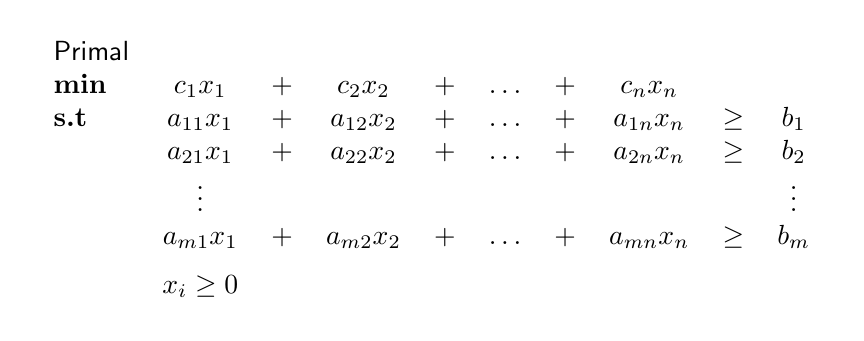
\begin{tikzpicture}
\def\x{0}
\def\y{0}
\node[anchor=north west] (primal) at (\x, \y) {
\begin{tabular}{lcccccccccc}
\textsf{Primal} & & & & & & & & & \\
$\displaystyle \mathbf{min}$ & $c_1 x_1$ & $+$ & $c_2 x_2$ & $+$ & $\ldots$ & $+$ & $c_n x_n$ & & \\
\textbf{s.t} & $a_{11} x_1$ & $+$ & $a_{12} x_2$ & $+$ & $\ldots$ & $+$ & $a_{1n} x_n$ & $\geq$ & $b_1$ \\
             & $a_{21} x_1$ & $+$ & $a_{22} x_2$ & $+$ & $\ldots$ & $+$ & $a_{2n} x_n$ & $\geq$ & $b_2$ \\
             & $\vdots$ & & & & & & & & $\vdots$ \\
             & $a_{m1} x_1$ & $+$ & $a_{m2} x_2$ & $+$ & $\ldots$ & $+$ & $a_{mn} x_n$ & $\geq$ & $b_m$ \\[0.2cm]
& $x_i \geq 0$ & & & & & & & &
\end{tabular}
};
\end{tikzpicture}
\end{center}

whose dual is easily shown to be

\begin{center}
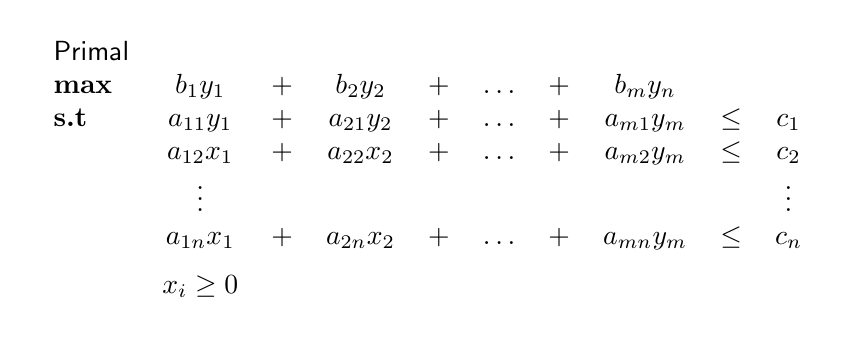
\begin{tikzpicture}
\def\x{0}
\def\y{0}
\node[anchor=north west] (primal) at (\x, \y) {
\begin{tabular}{lcccccccccc}
\textsf{Primal} & & & & & & & & & \\
$\displaystyle \mathbf{max}$ & $b_1 y_1$ & $+$ & $b_2 y_2$ & $+$ & $\ldots$ & $+$ & $b_m y_n$ & & \\
\textbf{s.t} & $a_{11} y_1$ & $+$ & $a_{21} y_2$ & $+$ & $\ldots$ & $+$ & $a_{m1} y_m$ & $\leq$ & $c_1$ \\
             & $a_{12} x_1$ & $+$ & $a_{22} x_2$ & $+$ & $\ldots$ & $+$ & $a_{m2} y_m$ & $\leq$ & $c_2$ \\
             & $\vdots$ & & & & & & & & $\vdots$ \\
             & $a_{1n} x_1$ & $+$ & $a_{2n} x_2$ & $+$ & $\ldots$ & $+$ & $a_{mn} y_m$ & $\leq$ & $c_n$ \\[0.2cm]
& $x_i \geq 0$ & & & & & & & &
\end{tabular}
};
\end{tikzpicture}
\end{center}

In general, we need a better way
for finding a new variable to introduce. In the previous example we did it by iterating over all remaining variables
and checking the corresponding constraint. Since CG is a framework that we want to use when we have a \emph{huge} amount of 
variables, this process is not realistic as it will involve checking the same amount of constraints. The idea to overcome this
is to express the problem of finding the variable as a another optimization problem which hopefully translates into something
that is solvable by an algorithm that is faster than a simple brute-force iterations on the missing variables.

The first step to achieve this is to express the condition for a new variable to be a candidate mathematically. Keeping the notation
used in the example, we see that each variable $x_i$ is associated to a column of coefficients $c_i, a_{1i}, a_{2i}, \ldots, a_{mi}$
where the first is the objective function coefficient and the others are the constraints coefficients in the primal.
The constraint associated to $x_i$ is the dual is given by
$$
a_{1i} + a_{2i} + \ldots + a_{mi} = \sum_{j = 1}^m a_{ji} y_i \leq c_i.
$$
Checking whether it is violated, or in other words, whether $x_i$ needs to be considered in the \textsf{Primal}, consists of 
checking whether
$$
\sum_{j = 1}^m a_{ji} y_i > c_i \Leftrightarrow \sum_{j = 1}^m a_{ji} y_i - c_i > 0.
$$

If we let $I$ be the set of indexes of the variables that we consider at a given point in the \textsf{Primal}, then the problem
of finding a new variable can be expressed as finding $i \in \{ 1, \ldots, n\} \setminus I$ such that
$$
\sum_{j = 1}^m a_{ji} y_i - c_i > 0.
$$
Therefore, if we compute the index $i^* \in \{ 1, \ldots, n\} \setminus I$ for which the value
$$
\sum_{j = 1}^m a_{ji^*} y_{i^*} - c_{i^*}
$$
is \emph{maximum} we know that there exists a new variable that we need to consider if and only if
$$
\sum_{j = 1}^m a_{ji^*} y_{i^*} - c_{i^*} > 0.
$$

Therefore, we can solve the problem of finding a new variable to add by solving the problem
$$
\max_{i \in \{ 1, \ldots, n\} \setminus I} \quad \sum_{j = 1}^m a_{ji} y_{i} - c_{i}.
$$
At first sight this problem might not seem any easier to solve than iterating over all $i \in \{ 1, \ldots, n\} \setminus I$
and computing the maximum but in practice this problem ofter has a nice structure and is usually solvable 
by a better, more efficient, algorithm than a simple brute force iteration. This problem is often referred to as the
\emph{pricing problem}.

Figure \ref{fig:col-gen-schema} provides a schematic vision of the column generation process.
CG generation is a very wide field and what we described here is just a very small glimpse into it \cite{desaulniers2006column}.
It is also important to note that what we did here only applies to \emph{continuous} linear programs and not to integer programming.
Therefore, we can only use this to compute solutions of LP that contain no integer variables. In order to obtain optimal
integral solution we need to add another layer to the algorithm and perform, for instance, a branch-and-price \cite{branchPrice}.
We did not explore this in this thesis but we believe that it would be interesting future work to see how fast we can
compute optimal solutions using this approach. 

In this thesis we instead use an heuristic algorithm to round the fractional solution getting an approximated solution rather
than an optimal one. %\todo{maybe we are going to explain branch-and-? also, if we find our notes}

\begin{figure}
\begin{center}
\begin{tikzpicture}
\node[draw, rounded corners, inner sep=0.25cm] (start) at (0, 0) {
  \begin{varwidth}{4cm}
    Select an initial set of variables $I$ such that \textsf{Primal}($I$)
    is feasible.
  \end{varwidth}
};

\node[draw, below= 1cm of start, rounded corners, inner sep=0.25cm] (lpsolve) {
  \begin{varwidth}{4cm}
    Solve \textsf{Primal}($I$) obtaining the primal and dual solutions $x^*, y^*$
  \end{varwidth}
};

\node[draw, below= 1cm of lpsolve, rounded corners, inner sep=0.25cm] (pricing) {
  \begin{varwidth}{4cm}
    Compute $i^* \in \{ 1, \ldots, n\} \setminus I$ such that $\sum_{j = 1}^m a_{ji} y_{i} - c_{i}$
    is maximum
  \end{varwidth}
};


\node[draw, right= 4cm of pricing, rounded corners, inner sep=0.25cm] (add) {
  \begin{varwidth}{4cm}
    Add $i^*$ to $I$
  \end{varwidth}
};

\node[draw, below= 2cm of pricing, rounded corners, inner sep=0.25cm] (quit) {
  \begin{varwidth}{4cm}
    $x^*$ with is the optimal solution of \textsf{Primal} (with value $0$ on
    variables outside of $I$)
  \end{varwidth}
};


\draw[line width=2] (start) edge[->] (lpsolve);

\draw[line width=2] (lpsolve) edge[->] (pricing);

\draw[line width=2] (pricing) edge[->, above] node {$\sum_{j = 1}^m a_{ji} y_{i} - c_{i} > 0$} (add);
\draw[line width=2] (add) -- ++(0, 2.65) edge[->] (lpsolve);

\draw[line width=2] (pricing) edge[->]  node[anchor=west] {$\sum_{j = 1}^m a_{ji} y_{i} - c_{i} \leq 0$} (quit);

\end{tikzpicture}
\end{center}
\caption{The CG framework used in this thesis.}
\label{fig:col-gen-schema}
\end{figure}

\section{CG for the path model}

We apply the process that we described above to the path model for the TE problem. As we mentioned before,
this model has a huge amount of variables since we have one variable per sr-path in $\Pk$ and $|\Pk| = O(|G|^k)$. Recall that 
the path model is obtained by replacing $\PB$ by $\Pk$ on the formulation of \bhatia.

\begin{center}
\begin{tabular}{crcllr}
\multicolumn{5}{l}{$\srtepath(G, \mathcal{D})$} \\[0.5cm] 
$\displaystyle \mathbf{min} \quad \lambda$ & & & & & \\[0.5cm]
$\textbf{s.t.}$ & $\displaystyle \sum_{\sr{p} \in \Pk} x_{d \sr{p}}$ & $=$ & $1$ & $\forall d \in \mathcal{D}$ \\[0.5cm] 
& $\displaystyle \sum_{\sr{p} \in \Pk} \sum_{d \in \mathcal{D}} \r(\sr{p}, e)  \cdot \vol(d) \cdot x_{d \sr{p}}$ & $\leq$ & $\lambda \cdot \bnd(e)$ & $\forall e \in E(G)$ \\[0.5cm]
& $x_{d\sr{p}} \in \{ 0, 1 \}$ & & & $\forall \sr{p} \in \Pk, \ \forall d \in \mathcal{D}$
\end{tabular}
\end{center}

Our experiments showed that working directly on the path model caused the column generation process described in Figure \ref{fig:col-gen-schema}
to require adding a lot of columns before proving optimality. It would get stuck with the same optimal value for the restricted problem
for huge number of iterations. For this reason we decided to formulate the problem with the same constraints but with the objective of routing
a maximum amount of demands for a given factor $\lambda$.

Since $x_{d \sr{p}}$ says whether demand $d$ is routed over sr-path $\sr{p}$, the total amount of traffic that is routed by a solution $x_{d\sr{p}}$ 
if given 
$$
\sum_{\sr{p} \in \Pk} \sum_{d \in \mathcal{D}} \vol(d) \cdot x_{d\sr{p}}.
$$

Routing a maximum demand volume thus amounts at maximizing this value. Putting it together with the constraints from the path model \srtepath~we obtain the 
following model.

\begin{center}
\begin{tabular}{crcll}
\multicolumn{5}{l}{$\displaystyle \srtepathdem(G, \mathcal{D}, \mathcal{P}, \lambda)$} \\[0.5cm] 
$\displaystyle \mathbf{max}$ & $\displaystyle \sum_{\sr{p} \in \Pk} \sum_{d \in \mathcal{D}} \vol(d) \cdot x_{dp}$ & & & \\[0.5cm]
$\textbf{s.t.}$ & $\displaystyle \sum_{\sr{p} \in \Pk} x_{d \sr{p}}$ & $\leq$ & $1$ & $\forall d \in \mathcal{D}$ \\[0.5cm] 
& $\displaystyle \sum_{\sr{p} \in \Pk} \sum_{d \in \mathcal{D}} \r(\sr{p}, e)  \cdot \vol(d) \cdot x_{d \sr{p}}$ & $\leq$ & $\lambda \cdot \bnd(e)$ & $\forall e \in E(G)$ \\[0.5cm] 
& $x_{d \sr{p}} \in \{0, 1\}$ & $\geq$ & $0$ & $\forall \sr{p} \in \Pk, \ \forall d \in \mathcal{D}$
\end{tabular}
\end{center}



In this formulation, $\lambda$ is a parameter that is given as input. We still want to minimize it so that we end up with a solution of Problem \ref{prob:srte}. However, we do not do this directly with linear programming, we instead perform a binary search on $\lambda$ to find the minimum lambda that is able to route \emph{all} demands.
The other difference relative to the original path model is that on the first set of constraints we now have an inequality rather than an equality. Both are equivalent.
This is the the case because, since the objective now is to route the maximum amount of demands, we always end up with a solution that selects one path per demand. The only reason for using
the inequality is that it simplifies a bit the process of finding the dual.

We apply the process described in our CG introduction to this problem. Since CG needs a LP and \srtepathdem~is a MIP, we first relax integrality constraints  
by replacing $x_{d \sr{p}} \in \{ 0, 1 \}$ by $x_{d \sr{p}} \geq 0$. Note that, again, the most natural would have been to say $x_{d \sr{p}} \in [0, 1]$ but saying $x_{d \sr{p}} \geq 0$ is equivalent
for this problem because of the first set of constraints. The reason for this choice is again that is makes the process of computing the dual simpler because it leaves the 
formulation in a standard form. We also need to add the current set of variables as a parameter. Since in our case variables correspond to sr-paths, we pass
as an argument a set of sr-paths $\mathcal{P}$ corresponding to the set of variables to which we restrict the problem. The CG process then slowly grow this
set until we reach an optimal solution. The linear programming relaxation we obtain is the following.

\begin{center}
\begin{tabular}{crcll}
\multicolumn{5}{l}{$\displaystyle \srtepathlp(G, \mathcal{D}, \mathcal{P}, \lambda)$} \\[0.5cm] 
$\displaystyle \mathbf{max}$ & $\displaystyle \sum_{\sr{p} \in \Pk} \sum_{d \in \mathcal{D}} \vol(d) \cdot x_{dp}$ & & & \\[0.5cm]
$\textbf{s.t.}$ & $\displaystyle \sum_{\sr{p} \in \Pk} x_{d \sr{p}}$ & $\leq$ & $1$ & $\forall d \in \mathcal{D}$ \\[0.5cm] 
& $\displaystyle \sum_{\sr{p} \in \Pk} \sum_{d \in \mathcal{D}} \r(\sr{p}, e)  \cdot \vol(d) \cdot x_{d \sr{p}}$ & $\leq$ & $\lambda \cdot \bnd(e)$ & $\forall e \in E(G)$ \\[0.5cm] 
& $x_{d\sr{p}}$ & $\geq$ & $0$ & $\forall \sr{p} \in \Pk, \ \forall d \in \mathcal{D}$
\end{tabular}
\end{center}

Since $\srtepathlp$ is already in standard form it is very easy to obtain its dual. In general, computing the dual
of a linear program can be achieved by following a systematic procedure. We omit the details here as this is quite a common process.
Doing so we obtain the following formulation for the dual.

\begin{center}
\begin{tabular}{crcll}
\multicolumn{5}{l}{$\displaystyle \srtepathlpdual(G, \mathcal{D}, \mathcal{P}, \lambda)$} \\[0.5cm] 
$\displaystyle \mathbf{min}$ & $\displaystyle \lambda \cdot \sum_{e \in E(G)} \bnd(e) \cdot y_e + \sum_{d \in \mathcal{D}} z_d$ & & & \\[0.5cm]
$\textbf{s.t.}$ & $z_d + \sum_{e \in E(G)} \r(\sr{p}, e) \cdot \vol(d) \cdot y_e$ & $\geq$ & $\vol(d)$ & $\forall \sr{p} \in \Pk$ \\[0.5cm] 
& $y_e, z_d$ & $\geq$ & $0$ & $\forall \sr{p} \in \Pk, \ \forall d \in \mathcal{D}$
\end{tabular}
\end{center}

The next step is to describe the pricing problem. By what we said above, this  corresponds to finding a sr-path $\sr{p} \in \Pk$ and a demand $d \in \mathcal{D}$
that violate the dual constraints, that is, such  that
\begin{align*}
z_d + \sum_{e \in E(G)} \r(\sr{p}, e) \cdot \vol(d) \cdot y_e < \vol(d) & \Leftrightarrow \\
\sum_{e \in E(G)} \r(\sr{p}, e) \cdot \vol(d) \cdot y_e < \vol(d) - z_d & \Leftrightarrow \\
\sum_{e \in E(G)} \r(\sr{p}, e) \cdot y_e < \frac{\vol(d) - z_d}{\vol(d)} & \\
\end{align*}
If such $\sr{p}$ and $d$ exist then we will add $\sr{p}$ to the $\mathcal{P}$. If not, then, by what we said above, we know that the optimal solution for the restricted sr-path set $\mathcal{P}$
is also optimal for the complete sr-path set $\Pk$.

\begin{problem}{SRTE pricing}
\label{prob:srte-pricing}
\textbf{Input:} A network $G$, a demand set $\mathcal{D}$, $k \geq \mathbb{N}$ and values $y_e \geq 0$ for each $e \in E(G)$.

\textbf{Output:} A sr-path $\sr{p} \in \Pk$ and a demand $d \in \mathcal{D}$ such that
$$
\sum_{e \in E(G)} \r(\sr{p}, e) \cdot y_e < \frac{\vol(d) - z_d}{\vol(d)}
$$
or report that no such path exists.
\end{problem}

\begin{theorem}
Problem \ref{prob:srte-pricing} can be solved in polynomial time. 
\end{theorem}

\begin{proof}
Let $d \in \mathcal{D}$.
Consider the sr-metric $c$ defined for all $u, v \in V(G)$ and $e \in E(G)$ as
$$
c(u, v) = \sum_{e \in E(G)} \r(u, v, e) \cdot y_e
$$
and
$$
c(e) = y_e.
$$
Let know that we can compute a sr-path $\sr{p} = \langle x_1, \ldots, x_l \rangle \in \Pk$ that minimizes
$$
c(\sr{p}) = \sum_{i = 2}^l c(x^2_{i - 1}, x^1_i) + \sum_{i : x_i \in E(G)} c(x_i)
$$
in polynomial time using Algorithm \ref{algo:min_weight_sr_path} from Chapter \ref{chapter:sr-optimal}. We have that
\begin{align*}
c(\sr{p}) & = \sum_{i = 2}^l c(x^2_{i - 1}, x^1_i) + \sum_{i : x_i \in E(G)} c(x_i) \\
& = \sum_{i = 2}^l  \sum_{e \in E(G)} \r(x^2_{i - 1}, x^1_i, e) \cdot y_e + \sum_{i : x_i \in E(G)} y_{x_i} \\
& = \sum_{e \in E(G)} \sum_{i = 2}^l \r(x^2_{i - 1}, x^1_i, e) \cdot y_e + \sum_{e \in E(G)} \sum_{i : x_i = e} y_{e} \\
& = \sum_{e \in E(G)} \left( \sum_{i = 2}^l \r(x^2_{i - 1}, x^1_i, e) \cdot y_e + \sum_{i : x_i = e} y_{e} \right) \\
& = \sum_{e \in E(G)} \left( \sum_{i = 2}^l \r(x^2_{i - 1}, x^1_i, e) + \sum_{i : x_i = e} 1 \right) \cdot y_e \\
& = \sum_{e \in E(G)} \r(\sr{p}, e)\cdot y_e.
\end{align*}
Since $\sr{p}$ has minimum cost, Problem \ref{prob:srte-pricing} has a solution if and only if
$$
c(\sr{p}) =  \sum_{e \in E(G)} \r(\sr{p}, e)\cdot y_e < \frac{\vol(d) - z_d}{\vol(d)}
$$
in which case $\sr{p}$ is a solution. Since Algorithm \ref{algo:min_weight_sr_path} runs in polynomial time, this means that
we can decide in polynomial time whether for a given demand $d \in \mathcal{D}$ there exists a sr-path $\sr{p}$ that violates the dual constraints.
Thus by iterating over all demands we get a polynomial time algorithm overall.
\end{proof}

With this theorem we have an example of a problem where finding a new variable to add can be done in a much more efficient way
than iterating over all remaining variables. Using the schema in Figure \ref{fig:col-gen-schema} we can then compute optimal
solutions to the LP relaxation \srtepathlp~of \srtepathdem.

The solution obtained with this process is optimal for Problem \ref{prob:srte-mul} and provides a lower bound form Problem \ref{prob:srte}.
In itself this is already a good result since those bounds are important for evaluating the quality of greedy solution. Until now, the
best lower bounds were computed using the MCF. The bounds obtained with the MCF are of lower quality since they do not take into account
segment routing as show at the end of this chapter.

\section{Minimizing the worst link utilization $\lambda$}

We saw in the previous section how to use CG to compute the maximum demand volume that we can route for a given 
capacity factor $\lambda$. In this section we explain how to use this as a sub-routine to compute the
minimum $\lambda$ for which we can route \emph{all} demands.

Let $\mathcal{V} = \sum_{d \in \mathcal{D}} \vol(d)$ be the total volume of demands in $\mathcal{D}$. To find the minimum
capacity factor perform a binary search on $\lambda \in [0, \lambda_M]$ where $\lambda_M$ is a big enough capacity factor
that ensure that all demands can be routed. For each $\lambda$ we solve $\srtepathdem(G, \mathcal{D}, P, \lambda)$. If the
solution is $\mathcal{V}$ then we continue the search with $\lambda$ as the new upper bound. Otherwise we set $\lambda$
as the new lower bound and continue. Each time we solve $\srtepathdem(G, \mathcal{D}, P, \lambda)$ we do not start from scratch. 
We continue the CG process with the set of paths $P$ from the previous iterations.

\subsubsection*{Initial sr-path set}

We need to select an initial feasible sr-path set $\mathcal{P}$. In this case, feasibility
is not an issue as we can select the capacity factor $\lambda_M$ so that it is large enough to make any solution with at least one sr-path per demand
feasible. To compute the initial path set, we use Algorithm \ref{algo:max_cap_sr_path} to compute the maximum capacity sr-path for each demand.

% For this reason we choose to use to start the algorithm with $\mathcal{P} = \left\{ \langle s, t \rangle \mid (s, t, \nu) \in \mathcal{D} \right\}$.
% Using an heuristic algorithm for selecting a better path set might improve the runtime of the algorithm. We did not explore this further in this thesis
% but we encourage people to do so if they want to implement this approach on real network. \todo{actually we did try the maximum capacity paths, should we talk about that?
% maybe in the min lat path chapter we can add some more stuff explaining how we can compute this}

\subsubsection*{Generating new paths}

We explained above that we can solve the pricing by iterating over all demands $d \in \mathcal{D}$ and computing a minimum cost sr-path for
specific weights that depend on the values $y, z$ of the dual solution. There might be several sr-path demand pairs $\sr{p}, d$ that violate
 the dual constraints and each such path corresponds to a new candidate variable that might improve the current solution if added. However,
if there are a lot of demands, computing the minimum cost sr-path for each and every one of them may be time consuming, even being a polynomial time procedure. Also, adding a lot of new paths
makes solving the relaxed problem slower since it will contain more variables. On the other hand, having more paths will maybe make the CG converge faster 
towards the optimal solution. Hence, we face a trade-off between adding more paths and making each iteration slower or adding fewer paths and having more iterations overall.

To have more control over this, we add a parameter to our algorithm $maxp$ that limits the number of sr-paths than can be generated in a single iteration.
At each CG iteration we loop over all the demands and for each of them check if it has a sr-path to be added. After $maxp$ demands yield a new sr-path we stop this iteration
and solve the new linear program obtained by adding these paths. The order in which we iterate over the demands should be such that we start with demands that have a higher
chance of yielding a sr-path that violates the dual constraints, that is, a sr-path $\sr{p}$ such that

$$
\sum_{e \in E(G)} \r(\sr{p}, e) \cdot y_e < \frac{\vol(d) - z_d}{\vol(d)}.
$$

Hence, we sort the demands by decreasing value of $\frac{\vol(d) - z_d}{\vol(d)}$ since the higher this value is, the more likely we are of finding a
sr-path whose weight lower cost. This is important since it helps avoiding useless time consuming invocations of the minimum cost sr-path algorithm.

\subsubsection*{Rounding heuristic}

As we explained above, at the end of the column generation process, we have an optimal solution for the relaxed master problem $\srtepathlp$ where variables can have fractional
values. In practice, this means that each demand might be split over several paths, in other words, we have an optimal segment routing solution for Problem \ref{prob:srte-mul}.
If we seek a solution from Problem \ref{prob:srte} we need to ensure that each demand is assigned to exactly one path. If sub-optimal solutions are acceptable, then an efficient
way to achieve this is to use some kind of heuristic to assign a path to each demand amongst the paths obtained in the end. We propose to do this by re-solving 
$\srtepath$ with integrality constraints using a MIP solver. As we discuss later, our experiments showed that in this way we obtain near optimal solutions to Problem \ref{prob:srte}.
This is an heuristic since, with integer variables, there is no guarantee that the restricted optimal solution is the optimal for the unrestricted problem.

By putting all these ideas together we can provide the following formal description of our column generation algorithm for the traffic engineering problem.
Algorithm \ref{algo:iterate} performs one iteration of the column generation algorithm. It starts on line \ref{line:mastersolve} by computing the optimal solution of the linear program
$\srtepathlp$ for the current sr-path set obtaining a primal solution $x$, the corresponding dual solution $y, z$ and the maximum value $vol$ that we can be routed on the current path set for the current capacity factor $\lambda$. Afterwards, from line \ref{line:coststart} to line \ref{line:costend} it computes the sr-metric used for the minimum cost sr-path computation. Then it iterates over all
demands and tries to find new paths to add. All those paths are put together and returned.

Algorithm \ref{algo:colgen} performs column generation iterations by calling Algorithm \ref{algo:iterate} until no new paths are found thus computing an optimal solution of 
$\srtepathlp(\mathcal{P}, \mathcal{D}, \lambda)$ for a given capacity factor $\lambda$ over the full sr-path set $\Pk$. Finally, Algorithm \ref{algo:SRGen} uses the column generation as a sub-routine 
on a binary search to find the smallest value of $\lambda$ such that the optimal solution of $\srtepathlp(\mathcal{P}, \mathcal{D}, \lambda)$ is equal to $\mathcal{V}$. In other words, it uses a binary
search combined with the column generation to find the smallest capacity factor that allows one to route the whole volume of demands.

\begin{algorithm}[t]
\small
\caption{$\textsf{iterate-CG}\left( G, \mathcal{P}, \mathcal{D}, \lambda, \textit{maxp} \right)$}
\begin{algorithmic}[1]
%\algrule
\STATE $x, (y, z)_x, \textit{vol} \gets \textsf{LP-solve}(\srtepathlp(\mathcal{P}, \mathcal{D}, \lambda))$ \label{line:mastersolve}
\FOR{$x, y \in V$} \label{line:coststart}
  \STATE $c(x, y) \gets \sum_{e \in E(\langle x, y \rangle)} \r(x, y, e) \cdot y_e$           
\ENDFOR
\FOR{$e \in E$}
  \STATE $c(e) \gets y_e$
\ENDFOR \label{line:costend}
\STATE $P' \gets \emptyset$
\FOR{$d \in \mathcal{D}$ \textbf{in decreasing order of $(\vol(d) - z_d) \slash \vol(d)$}}
  \STATE $p \gets \textsf{mincost-srpath}(s(d), t(d), c)$
  \IF{$c(p) < (v(d) - \delta_d) \slash v$}
    \STATE $P' \gets P' \cup \{ p \}$
  \ENDIF
  \IF{$|P'| \geq \textit{maxp}$}
    \STATE \textbf{break}
  \ENDIF
\ENDFOR
\RETURN $P'$
\end{algorithmic}
\label{algo:iterate}
\end{algorithm}

\begin{algorithm}[t]
\small
\caption{$\textsf{binsearch-CG}\left( \mathcal{D}, \lambda_M, k, \epsilon, \textit{maxp} \right)$}
\begin{algorithmic}[1]
%\algrule
\STATE $\mathcal{P} \gets \{ \textsf{maxCapSrPath}(g, \tau, s, t, k) \mid (s, t, d) \in \mathcal{D} \}$ \label{line:init}
\STATE $\mathcal{V} \gets \sum_{d \in \mathcal{D}} \vol(d)$
\STATE $lb \gets 0$
\STATE $ub \gets \lambda_M$
\WHILE{$|lb - ub| > \epsilon$}
  \STATE $\lambda \gets (lb + ub) \slash 2$
  \STATE $x, (y, z)_x, \textit{vol} \gets \textsf{column-generation}(\mathcal{P}, \mathcal{D}, \lambda, \textit{maxp})$
  \IF{$\textit{vol} = \mathcal{V}$}
    \STATE $lb \gets \lambda$
  \ELSE
    \STATE $ub \gets \lambda$
  \ENDIF
\ENDWHILE
\RETURN $\textsf{ILP-solve}(\srtepathdem(\mathcal{P}, \mathcal{D}))$ 
\end{algorithmic}
\label{algo:SRGen}
\end{algorithm}

\begin{algorithm}[t]
\small
\caption{$\textsf{column-generation}\left( \mathcal{P}, \mathcal{D}, \lambda, \textit{maxp} \right)$}
\begin{algorithmic}[1]
%\algrule
\WHILE{$P' \gets \textsf{iterate}(\mathcal{P}, \mathcal{D}, \lambda, \textit{maxp}) \neq \emptyset$}
  \STATE $\mathcal{P} \gets \mathcal{P} \cup P'$
\ENDWHILE
%\STATE $\primalx = \textsf{ILP-solve}(\primal(\P, \D, \lambda))$
\RETURN $\textsf{LP-solve}(\srtepathdem(G, \mathcal{D}, \mathcal{P}, \lambda))$
\end{algorithmic}
\label{algo:colgen}
\end{algorithm}


\section{Pinpointing single-link failures}

In this section we explain how to use a sr-cycle cover to detect single-link failures.

As mentioned in the introduction of this chapter, the idea is to have node $s$ 
regularly send monitoring probes over the sr-cycles of in a sr-cycle cover $C \subseteq \Csk$. Since we are using sr-cycles,
if the network is operating without failures, each probe must eventually come back to the vantage point $s$.
If at least one such probe does not come back, we know that at least one of the edges in the cycle associated with it
has a failure. We refer to the sr-cycles in the cycle cover $C$ as \emph{probing cycles}.

Let $\sr{c}$ be a cycle with a failure, that is, whose probe did not return. 
Because we use deterministic cycles, if we map $\sr{c}$ back to $G$, we get a cycle $c = (e_1, e_2, \ldots, e_l)$.
Recall that in this chapter we assume that the network $G$ is symmetric so that for each edge $e$ there is a reverse edge $\rev(e)$ and that
$\igp$ is symmetric if $\igp(e) = \rev(\igp(e))$.
The idea to detect the failure is to perform a binary search to find the largest $i$ such that
the cycle $c_i = (e_1, \ldots, e_i, \rev(e_i), \ldots, \rev(e_1))$ contains no failure. For each $i$ we send another 
probe over $c_i$ and check whether it comes back. If it does, then we know that the index we seek is greater than or equal to $i$. 
If it does not then the index must be strictly smaller than $i$. The single-link failure assumption is important for this process to work.
Because the probe did not cycle back, we know that one of 
$e_1, \ldots, e_l$ is faulty. Therefore, since we assume single-link
failure, we know that each reverse edge is not faulty. Hence, when we send a binary search probe on $c_i$, if it does not come back,
we know that the problem is in one of $e_1, \ldots, e_i$. We refer to these sr-cycles as \emph{identification cycles}.

Figure \ref{fig:bs-srcycle_new} illustrates this on an example with $l = 8$ and the failure is on edge $e_5$. We start the search with $i = 4$. The green dotted path
illustrates that the probe successfully returned to $v_1$. Thus we know that edges $e_1, e_2$ and $e_3$ are up.
The search will select $i = 6$ and this time the probe did not return. We conclude that the error is either in $e_4$ or $e_5$.
Finally, we send a probe on $c_5$ which returns. We finally conclude that the problem is on link $e_5$.

\begin{figure}
\begin{center}
\begin{tabular}{cc}
\begin{tikzpicture}[scale=0.75]
\node[scale=0.15] (a) at (3.000, 0.000) {\router{$v_1$}{router}};
\node[scale=0.15] (b) at (2.121, 2.121) {\router{$v_2$}{router}};
\node[scale=0.15] (c) at (0.000, 3.000) {\router{$v_3$}{router}};
\node[scale=0.15] (d) at (-2.121, 2.121) {\router{$v_4$}{router}};
\node[scale=0.15] (e) at (-3.000, 0.000) {\router{$v_5$}{router}};
\node[scale=0.15] (f) at (-2.121, -2.121) {\router{$v_6$}{router}};
\node[scale=0.15] (g) at (-0.000, -3.000) {\router{$v_7$}{router}};
\node[scale=0.15] (h) at (2.121, -2.121) {\router{$v_8$}{router}};

\draw[line width=2] (a) edge[above, sloped, bend right, ->] node[black,font=\bfseries] {\footnotesize \texttt{$e_1$}} (b);
\draw[line width=2] (b) edge[above, sloped, bend right, ->] node[black,font=\bfseries] {\footnotesize \texttt{$e_2$}} (c);
\draw[line width=2] (c) edge[above, sloped, bend right, ->] node[black,font=\bfseries] {\footnotesize \texttt{$e_3$}} (d);
\draw[line width=2] (d) edge[above, sloped, bend right, ->] node[black,font=\bfseries] {\footnotesize \texttt{$e_4$}} (e);
\draw[line width=2] (e) edge[below, sloped, bend right, ->] node[black,font=\bfseries] {\footnotesize \texttt{$e_5$}} (f);
\draw[line width=2] (f) edge[below, sloped, bend right, ->] node[black,font=\bfseries] {\footnotesize \texttt{$e_6$}} (g);
\draw[line width=2] (g) edge[below, sloped, bend right, ->] node[black,font=\bfseries] {\footnotesize \texttt{$e_7$}} (h);
\draw[line width=2] (h) edge[below, sloped, bend right, ->] node[black,font=\bfseries] {\footnotesize \texttt{$e_8$}} (a);
\draw (e) edge[sloped, bend right, ->] node[red, font=\bfseries] {\footnotesize \texttt{\Large \textsf{X}}} (f);

\draw[line width=2, gray] (a) edge[below, sloped, bend left, <-] node[gray,font=\bfseries] {\footnotesize \texttt{$\rev(e_1)$}} (b);
\draw[line width=2, gray] (b) edge[below, sloped, bend left, <-] node[gray,font=\bfseries] {\footnotesize \texttt{$\rev(e_2)$}} (c);
\draw[line width=2, gray] (c) edge[below, sloped, bend left, <-] node[gray,font=\bfseries] {\footnotesize \texttt{$\rev(e_3)$}} (d);
\draw[line width=2, gray] (d) edge[below, sloped, bend left, <-] node[gray,font=\bfseries] {\footnotesize \texttt{$\rev(e_4)$}} (e);
\draw[line width=2, gray] (e) edge[above, sloped, bend left, <-] node[gray,font=\bfseries] {\footnotesize \texttt{$\rev(e_5)$}} (f);

\draw[line width=2, gray] (f) edge[above, sloped, bend left, <-] node[gray,font=\bfseries] {\footnotesize \texttt{$\rev(e_6)$}} (g);
\draw[line width=2, gray] (g) edge[above, sloped, bend left, <-] node[gray,font=\bfseries] {\footnotesize \texttt{$\rev(e_7)$}} (h);
\draw[line width=2, gray] (h) edge[above, sloped, bend left, <-] node[gray,font=\bfseries] {\footnotesize \texttt{$\rev(e_8)$}} (a);

\draw[darkgreen, ultra thick, dotted, ->] plot [smooth] coordinates { ($(a)+(0.5,0)$) ($(b)+(0,0.5)$) ($(c)+(0,0.5)$) ($(d)+(0,0.5)$) ($(d)+(-0.5,0)$) ($(d)+(0,-0.5)$) ($(c)+(0,-0.5)$) ($(b)+(0,-0.5)$) ($(a)$) };

\end{tikzpicture}

&

\begin{tikzpicture}[scale=0.75]
\node[scale=0.15] (1) at (3.000, 0.000) {\router{$v_1$}{router}};
\node[scale=0.15] (2) at (2.121, 2.121) {\router{$v_2$}{router}};
\node[scale=0.15] (3) at (0.000, 3.000) {\router{$v_3$}{router}};
\node[scale=0.15] (4) at (-2.121, 2.121) {\router{$v_4$}{green}};
\node[scale=0.15] (5) at (-3.000, 0.000) {\router{$v_5$}{router}};
\node[scale=0.15] (6) at (-2.121, -2.121) {\router{$v_6$}{router}};
\node[scale=0.15] (7) at (-0.000, -3.000) {\router{$v_7$}{router}};
\node[scale=0.15] (8) at (2.121, -2.121) {\router{$v_8$}{router}};

\draw[line width=2, darkgreen] (1) edge[above, sloped, bend right, ->] node[black,font=\bfseries] {\footnotesize \texttt{$e_1$}} (2);
\draw[line width=2, darkgreen] (2) edge[above, sloped, bend right, ->] node[black,font=\bfseries] {\footnotesize \texttt{$e_2$}} (3);
\draw[line width=2, darkgreen] (3) edge[above, sloped, bend right, ->] node[black,font=\bfseries] {\footnotesize \texttt{$e_3$}} (4);
\draw[line width=2] (4) edge[above, sloped, bend right, ->] node[black,font=\bfseries] {\footnotesize \texttt{$e_4$}} (5);
\draw[line width=2] (5) edge[below, sloped, bend right, ->] node[black,font=\bfseries] {\footnotesize \texttt{$e_5$}} (6);
\draw[line width=2] (6) edge[below, sloped, bend right, ->] node[black,font=\bfseries] {\footnotesize \texttt{$e_6$}} (7);
\draw[line width=2] (7) edge[below, sloped, bend right, ->] node[black,font=\bfseries] {\footnotesize \texttt{$e_7$}} (8);
\draw[line width=2] (8) edge[below, sloped, bend right, ->] node[black,font=\bfseries] {\footnotesize \texttt{$e_8$}} (1);
\draw (5) edge[sloped, bend right, ->] node[red, font=\bfseries] {\footnotesize \texttt{\Large \textsf{X}}} (6);

\draw[line width=2, gray, darkgreen] (1) edge[below, sloped, bend left, <-] node[gray,font=\bfseries] {\footnotesize \texttt{$\rev(e_1)$}} (2);
\draw[line width=2, gray, darkgreen] (2) edge[below, sloped, bend left, <-] node[gray,font=\bfseries] {\footnotesize \texttt{$\rev(e_2)$}} (3);
\draw[line width=2, gray, darkgreen] (3) edge[below, sloped, bend left, <-] node[gray,font=\bfseries] {\footnotesize \texttt{$\rev(e_3)$}} (4);
\draw[line width=2, gray] (4) edge[below, sloped, bend left, <-] node[gray,font=\bfseries] {\footnotesize \texttt{$\rev(e_4)$}} (5);
\draw[line width=2, gray] (5) edge[above, sloped, bend left, <-] node[gray,font=\bfseries] {\footnotesize \texttt{$\rev(e_5)$}} (6);
\draw[line width=2, gray] (6) edge[above, sloped, bend left, <-] node[gray,font=\bfseries] {\footnotesize \texttt{$\rev(e_6)$}} (7);
\draw[line width=2, gray] (7) edge[above, sloped, bend left, <-] node[gray,font=\bfseries] {\footnotesize \texttt{$\rev(e_7)$}} (8);
\draw[line width=2, gray] (8) edge[above, sloped, bend left, <-] node[gray,font=\bfseries] {\footnotesize \texttt{$\rev(e_8)$}} (1);

\draw[red!50!black, ultra thick, dotted, ->] plot [smooth] coordinates { 
($(a)+(0.5,0)$) ($(b)+(0,0.5)$) ($(c)+(0,0.5)$) ($(d)+(0,0.5)$) ($(e)+(-0.5,0)$) ($(f)+(-0.5,0)$) 
($(f)+(0,-0.5)$) ($(f)+(0.5,0)$) ($(e)+(0.5,0)$) ($(d)+(0,-0.5)$) ($(c)+(0,-0.5)$) ($(b)+(0,-0.5)$) ($(a)$) 
};

\end{tikzpicture}

\\

\footnotesize

First step of binary search. Success.

&

\footnotesize

Second step of binary search. Failure.

\\

\footnotesize

Edges $e_1, e_2, e_3$ are up.

&

\footnotesize

One of $e_4, e_5$ is down.

\\[0.5cm]

\begin{tikzpicture}[scale=0.75]
\node[scale=0.15] (1) at (3.000, 0.000) {\router{$v_1$}{router}};
\node[scale=0.15] (2) at (2.121, 2.121) {\router{$v_2$}{router}};
\node[scale=0.15] (3) at (0.000, 3.000) {\router{$v_3$}{router}};
\node[scale=0.15] (4) at (-2.121, 2.121) {\router{$v_4$}{green}};
\node[scale=0.15] (5) at (-3.000, 0.000) {\router{$v_5$}{router}};
\node[scale=0.15] (6) at (-2.121, -2.121) {\router{$v_6$}{red!50!white}};
\node[scale=0.15] (7) at (-0.000, -3.000) {\router{$v_7$}{router}};
\node[scale=0.15] (8) at (2.121, -2.121) {\router{$v_8$}{router}};

\draw[line width=2, darkgreen] (1) edge[above, sloped, bend right, ->] node[black,font=\bfseries] {\footnotesize \texttt{$e_1$}} (2);
\draw[line width=2, darkgreen] (2) edge[above, sloped, bend right, ->] node[black,font=\bfseries] {\footnotesize \texttt{$e_2$}} (3);
\draw[line width=2, darkgreen] (3) edge[above, sloped, bend right, ->] node[black,font=\bfseries] {\footnotesize \texttt{$e_3$}} (4);
\draw[line width=2] (4) edge[above, sloped, bend right, ->] node[black,font=\bfseries] {\footnotesize \texttt{$e_4$}} (5);
\draw[line width=2] (5) edge[below, sloped, bend right, ->] node[black,font=\bfseries] {\footnotesize \texttt{$e_5$}} (6);
\draw[line width=2] (6) edge[below, sloped, bend right, ->] node[black,font=\bfseries] {\footnotesize \texttt{$e_6$}} (7);
\draw[line width=2] (7) edge[below, sloped, bend right, ->] node[black,font=\bfseries] {\footnotesize \texttt{$e_7$}} (8);
\draw[line width=2] (8) edge[below, sloped, bend right, ->] node[black,font=\bfseries] {\footnotesize \texttt{$e_8$}} (1);
\draw (5) edge[sloped, bend right, ->] node[red, font=\bfseries] {\footnotesize \texttt{\Large \textsf{X}}} (6);

\draw[line width=2, gray, darkgreen] (1) edge[below, sloped, bend left, <-] node[gray,font=\bfseries] {\footnotesize \texttt{$\rev(e_1)$}} (2);
\draw[line width=2, gray, darkgreen] (2) edge[below, sloped, bend left, <-] node[gray,font=\bfseries] {\footnotesize \texttt{$\rev(e_2)$}} (3);
\draw[line width=2, gray, darkgreen] (3) edge[below, sloped, bend left, <-] node[gray,font=\bfseries] {\footnotesize \texttt{$\rev(e_3)$}} (4);
\draw[line width=2, gray] (4) edge[below, sloped, bend left, <-] node[gray,font=\bfseries] {\footnotesize \texttt{$\rev(e_4)$}} (5);
\draw[line width=2, gray] (5) edge[above, sloped, bend left, <-] node[gray,font=\bfseries] {\footnotesize \texttt{$\rev(e_5)$}} (6);
\draw[line width=2, gray] (6) edge[above, sloped, bend left, <-] node[gray,font=\bfseries] {\footnotesize \texttt{$\rev(e_6)$}} (7);
\draw[line width=2, gray] (7) edge[above, sloped, bend left, <-] node[gray,font=\bfseries] {\footnotesize \texttt{$\rev(e_7)$}} (8);
\draw[line width=2, gray] (8) edge[above, sloped, bend left, <-] node[gray,font=\bfseries] {\footnotesize \texttt{$\rev(e_8)$}} (1);

\draw[darkgreen, ultra thick, dotted, ->] plot [smooth] coordinates { 
($(a)+(0.5,0)$) ($(b)+(0,0.5)$) ($(c)+(0,0.5)$) ($(d)+(0,0.5)$) ($(e)+(-0.5,0)$) 
($(e)+(0,-0.5)$) ($(e)+(0.5,0)$) ($(d)+(0,-0.5)$) ($(c)+(0,-0.5)$) ($(b)+(0,-0.5)$) ($(a)$) 
};

\end{tikzpicture}

&


\begin{tikzpicture}[scale=0.75]
\node[scale=0.15] (1) at (3.000, 0.000) {\router{$v_1$}{router}};
\node[scale=0.15] (2) at (2.121, 2.121) {\router{$v_2$}{router}};
\node[scale=0.15] (3) at (0.000, 3.000) {\router{$v_3$}{router}};
\node[scale=0.15] (4) at (-2.121, 2.121) {\router{$v_4$}{green}};
\node[scale=0.15] (5) at (-3.000, 0.000) {\router{$v_5$}{green}};
\node[scale=0.15] (6) at (-2.121, -2.121) {\router{$v_6$}{red!50!white}};
\node[scale=0.15] (7) at (-0.000, -3.000) {\router{$v_7$}{router}};
\node[scale=0.15] (8) at (2.121, -2.121) {\router{$v_8$}{router}};

\draw[line width=2, darkgreen] (1) edge[above, sloped, bend right, ->] node[black,font=\bfseries] {\footnotesize \texttt{$e_1$}} (2);
\draw[line width=2, darkgreen] (2) edge[above, sloped, bend right, ->] node[black,font=\bfseries] {\footnotesize \texttt{$e_2$}} (3);
\draw[line width=2, darkgreen] (3) edge[above, sloped, bend right, ->] node[black,font=\bfseries] {\footnotesize \texttt{$e_3$}} (4);
\draw[line width=2, darkgreen] (4) edge[above, sloped, bend right, ->] node[black,font=\bfseries] {\footnotesize \texttt{$e_4$}} (5);
\draw[line width=2] (5) edge[below, red!50!black, sloped, bend right, ->] node[black,font=\bfseries] {\footnotesize \texttt{$e_5$}} (6);
\draw[line width=2, opacity=0] (5) edge[red!50!black, sloped, bend right, ->] node (e5) {} (6);
\draw (5) edge[sloped, bend right, ->] node[red, font=\bfseries] {\footnotesize \texttt{\Large \textsf{X}}} (6);

\draw[line width=2] (6) edge[below, sloped, bend right, ->] node[black,font=\bfseries] {\footnotesize \texttt{$e_6$}} (7);
\draw[line width=2] (7) edge[below, sloped, bend right, ->] node[black,font=\bfseries] {\footnotesize \texttt{$e_7$}} (8);
\draw[line width=2] (8) edge[below, sloped, bend right, ->] node[black,font=\bfseries] {\footnotesize \texttt{$e_8$}} (1);

\draw[line width=2, gray, darkgreen] (1) edge[below, sloped, bend left, <-] node[gray,font=\bfseries] {\footnotesize \texttt{$\rev(e_1)$}} (2);
\draw[line width=2, gray, darkgreen] (2) edge[below, sloped, bend left, <-] node[gray,font=\bfseries] {\footnotesize \texttt{$\rev(e_2)$}} (3);
\draw[line width=2, gray, darkgreen] (3) edge[below, sloped, bend left, <-] node[gray,font=\bfseries] {\footnotesize \texttt{$\rev(e_3)$}} (4);
\draw[line width=2, gray, darkgreen] (4) edge[below, sloped, bend left, <-] node[gray,font=\bfseries] {\footnotesize \texttt{$\rev(e_4)$}} (5);
\draw[line width=2, gray, gray] (5) edge[above, sloped, bend left, <-] node[gray,font=\bfseries] {\footnotesize \texttt{$\rev(e_5)$}} (6);
%\draw[line width=2, gray, red!50!black, opacity=0] (5) edge[sloped, bend left, <-] node[gray,font=\bfseries] (re5) {} (6);


\draw[line width=2, gray] (6) edge[above, sloped, bend left, <-] node[gray,font=\bfseries] {\footnotesize \texttt{$\rev(e_6)$}} (7);
\draw[line width=2, gray] (7) edge[above, sloped, bend left, <-] node[gray,font=\bfseries] {\footnotesize \texttt{$\rev(e_7)$}} (8);
\draw[line width=2, gray] (8) edge[above, sloped, bend left, <-] node[gray,font=\bfseries] {\footnotesize \texttt{$\rev(e_8)$}} (1);

%\draw[darkgreen, ultra thick, dotted, ->] plot [smooth] coordinates { 
%($(a)+(0.5,0)$) ($(b)+(0,0.5)$) ($(c)+(0,0.5)$) ($(d)+(0,0.5)$) ($(e)+(-0.5,0)$) 
%($(e)+(0,-0.5)$) ($(e)+(0.5,0)$) ($(d)+(0,-0.5)$) ($(c)+(0,-0.5)$) ($(b)+(0,-0.5)$) ($(a)$) 
%};

%\node (fail) at (0, 0) {failure};

%\draw[->, dashed] (fail) -- (e5);
%\draw[->, dashed] (fail) -- (re5);


\end{tikzpicture}

\\

\footnotesize

Third step of binary search. Success.

&

\footnotesize

End of the search.

\\

\footnotesize

Edges $e_4$ is up.

&

\footnotesize

Failure detected in $e_5$.

\end{tabular}
\end{center}
\caption{Binary search to identify the failure (single-link failure assumption).}
\label{fig:bs-srcycle_new}
\end{figure}

To illustrate why the single link-failure assumption is important, let's see happens with this process
when multiple failures occur. Imagine the same example as in Figure \ref{fig:bs-srcycle_new} but assume that
edge $\rev(e_3)$ is also down. In this case the first binary search probe will fail to return and the search
will stop at $i = 3$ and the algorithm will say that the problem is on edge $e_3$. However $e_3$ is up
and it is $\rev(e_3)$ that prevents the probe to return. This shows that with multiple failures, we cannot
know exactly which link is down. However, we still can say that either $e_3$ is down \emph{or} $\rev(e_3)$ is
down. Figure \ref{fig:bs-srcycle_new2} illustrates this.

This means that in presence of multiple link failures, we cannot tell exactly which link is down but we can
still find a set of two links $\{ e, \rev(e) \}$ such that we are sure that at least one of them is down.

\begin{figure}
\begin{center}
\begin{tabular}{cc}
\begin{tikzpicture}[scale=0.75]
\node[scale=0.15] (a) at (3.000, 0.000) {\router{$v_1$}{router}};
\node[scale=0.15] (b) at (2.121, 2.121) {\router{$v_2$}{router}};
\node[scale=0.15] (c) at (0.000, 3.000) {\router{$v_3$}{router}};
\node[scale=0.15] (d) at (-2.121, 2.121) {\router{$v_4$}{router}};
\node[scale=0.15] (e) at (-3.000, 0.000) {\router{$v_5$}{router}};
\node[scale=0.15] (f) at (-2.121, -2.121) {\router{$v_6$}{router}};
\node[scale=0.15] (g) at (-0.000, -3.000) {\router{$v_7$}{router}};
\node[scale=0.15] (h) at (2.121, -2.121) {\router{$v_8$}{router}};

\draw[line width=2] (a) edge[above, sloped, bend right, ->] node[black,font=\bfseries] {\footnotesize \texttt{$e_1$}} (b);
\draw[line width=2] (b) edge[above, sloped, bend right, ->] node[black,font=\bfseries] {\footnotesize \texttt{$e_2$}} (c);
\draw[line width=2] (c) edge[above, sloped, bend right, ->] node[black,font=\bfseries] {\footnotesize \texttt{$e_3$}} (d);
\draw[line width=2] (d) edge[above, sloped, bend right, ->] node[black,font=\bfseries] {\footnotesize \texttt{$e_4$}} (e);
\draw[line width=2] (e) edge[below, sloped, bend right, ->] node[black,font=\bfseries] {\footnotesize \texttt{$e_5$}} (f);
\draw[line width=2] (f) edge[below, sloped, bend right, ->] node[black,font=\bfseries] {\footnotesize \texttt{$e_6$}} (g);
\draw[line width=2] (g) edge[below, sloped, bend right, ->] node[black,font=\bfseries] {\footnotesize \texttt{$e_7$}} (h);
\draw[line width=2] (h) edge[below, sloped, bend right, ->] node[black,font=\bfseries] {\footnotesize \texttt{$e_8$}} (a);
\draw (e) edge[sloped, bend right, ->] node[red, font=\bfseries] {\Large \textsf{X}} (f);

\draw[line width=2, gray] (a) edge[below, sloped, bend left, <-] node[gray,font=\bfseries] {\footnotesize \texttt{$\rev(e_1)$}} (b);
\draw[line width=2, gray] (b) edge[below, sloped, bend left, <-] node[gray,font=\bfseries] {\footnotesize \texttt{$\rev(e_2)$}} (c);
\draw[line width=2, gray] (c) edge[below, sloped, bend left, <-] node[gray,font=\bfseries] {\footnotesize \texttt{$\rev(e_3)$}} (d);
\draw[line width=2, gray] (d) edge[below, sloped, bend left, <-] node[gray,font=\bfseries] {\footnotesize \texttt{$\rev(e_4)$}} (e);
\draw[line width=2, gray] (e) edge[above, sloped, bend left, <-] node[gray,font=\bfseries] {\footnotesize \texttt{$\rev(e_5)$}} (f);
\draw[line width=2, gray] (c) edge[sloped, bend left, <-] node[red,font=\bfseries] {\Large \textsf{X}} (d);

\draw[line width=2, gray] (f) edge[above, sloped, bend left, <-] node[gray,font=\bfseries] {\footnotesize \texttt{$\rev(e_6)$}} (g);
\draw[line width=2, gray] (g) edge[above, sloped, bend left, <-] node[gray,font=\bfseries] {\footnotesize \texttt{$\rev(e_7)$}} (h);
\draw[line width=2, gray] (h) edge[above, sloped, bend left, <-] node[gray,font=\bfseries] {\footnotesize \texttt{$\rev(e_8)$}} (a);

\draw[red!50!black, ultra thick, dotted, ->] plot [smooth] coordinates { ($(a)+(0.5,0)$) ($(b)+(0,0.5)$) ($(c)+(0,0.5)$) ($(d)+(0,0.5)$) ($(d)+(-0.5,0)$) ($(d)+(0,-0.5)$) ($(c)+(0,-0.5)$) ($(b)+(0,-0.5)$) ($(a)$) };

\end{tikzpicture}

&

\begin{tikzpicture}[scale=0.75]
\node[scale=0.15] (1) at (3.000, 0.000) {\router{$v_1$}{router}};
\node[scale=0.15] (2) at (2.121, 2.121) {\router{$v_2$}{router}};
\node[scale=0.15] (3) at (0.000, 3.000) {\router{$v_3$}{router}};
\node[scale=0.15] (4) at (-2.121, 2.121) {\router{$v_4$}{red!50!white}};
\node[scale=0.15] (5) at (-3.000, 0.000) {\router{$v_5$}{router}};
\node[scale=0.15] (6) at (-2.121, -2.121) {\router{$v_6$}{router}};
\node[scale=0.15] (7) at (-0.000, -3.000) {\router{$v_7$}{router}};
\node[scale=0.15] (8) at (2.121, -2.121) {\router{$v_8$}{router}};

\draw[line width=2] (1) edge[above, sloped, bend right, ->] node[black,font=\bfseries] {\footnotesize \texttt{$e_1$}} (2);
\draw[line width=2] (2) edge[above, sloped, bend right, ->] node[black,font=\bfseries] {\footnotesize \texttt{$e_2$}} (3);
\draw[line width=2] (3) edge[above, sloped, bend right, ->] node[black,font=\bfseries] {\footnotesize \texttt{$e_3$}} (4);
\draw[line width=2] (4) edge[above, sloped, bend right, ->] node[black,font=\bfseries] {\footnotesize \texttt{$e_4$}} (5);
\draw[line width=2] (5) edge[below, sloped, bend right, ->] node[black,font=\bfseries] {\footnotesize \texttt{$e_5$}} (6);
\draw[line width=2] (6) edge[below, sloped, bend right, ->] node[black,font=\bfseries] {\footnotesize \texttt{$e_6$}} (7);
\draw[line width=2] (7) edge[below, sloped, bend right, ->] node[black,font=\bfseries] {\footnotesize \texttt{$e_7$}} (8);
\draw[line width=2] (8) edge[below, sloped, bend right, ->] node[black,font=\bfseries] {\footnotesize \texttt{$e_8$}} (1);
\draw (5) edge[sloped, bend right, ->] node[red, font=\bfseries] {\footnotesize \texttt{\Large \textsf{X}}} (6);

\draw[line width=2, gray] (1) edge[below, sloped, bend left, <-] node[gray,font=\bfseries] {\footnotesize \texttt{$\rev(e_1)$}} (2);
\draw[line width=2, gray] (2) edge[below, sloped, bend left, <-] node[gray,font=\bfseries] {\footnotesize \texttt{$\rev(e_2)$}} (3);
\draw[line width=2, gray] (3) edge[below, sloped, bend left, <-] node[gray,font=\bfseries] {\footnotesize \texttt{$\rev(e_3)$}} (4);
\draw[line width=2, gray] (4) edge[below, sloped, bend left, <-] node[gray,font=\bfseries] {\footnotesize \texttt{$\rev(e_4)$}} (5);
\draw[line width=2, gray] (5) edge[above, sloped, bend left, <-] node[gray,font=\bfseries] {\footnotesize \texttt{$\rev(e_5)$}} (6);
\draw[line width=2, gray] (6) edge[above, sloped, bend left, <-] node[gray,font=\bfseries] {\footnotesize \texttt{$\rev(e_6)$}} (7);
\draw[line width=2, gray] (7) edge[above, sloped, bend left, <-] node[gray,font=\bfseries] {\footnotesize \texttt{$\rev(e_7)$}} (8);
\draw[line width=2, gray] (8) edge[above, sloped, bend left, <-] node[gray,font=\bfseries] {\footnotesize \texttt{$\rev(e_8)$}} (1);
\draw[line width=2, gray] (c) edge[sloped, bend left, <-] node[red,font=\bfseries] {\Large \textsf{X}} (d);

\draw[darkgreen, ultra thick, dotted, ->] plot [smooth] coordinates 
{ ($(a)+(0.5,0)$) ($(b)+(0.5,0.5)$) ($(b)+(0,0.5)$) ($(b)+(-0.5,0)$)($(a)$) };

\end{tikzpicture}

\\

\footnotesize

First step of binary search. Failure.

&

\footnotesize

Second step of binary search. Success.

\\

\footnotesize

One of $e_1, e_2, e_3, \rev(e_3), \rev(e_2), \rev(e_1)$ is down.

&

\footnotesize

Edges $e_1, \rev(e_1)$ are up.

\\[0.5cm]

\begin{tikzpicture}[scale=0.75]
\node[scale=0.15] (1) at (3.000, 0.000) {\router{$v_1$}{router}};
\node[scale=0.15] (2) at (2.121, 2.121) {\router{$v_2$}{green}};
\node[scale=0.15] (3) at (0.000, 3.000) {\router{$v_3$}{router}};
\node[scale=0.15] (4) at (-2.121, 2.121) {\router{$v_4$}{red!50!white}};
\node[scale=0.15] (5) at (-3.000, 0.000) {\router{$v_5$}{router}};
\node[scale=0.15] (6) at (-2.121, -2.121) {\router{$v_6$}{router}};
\node[scale=0.15] (7) at (-0.000, -3.000) {\router{$v_7$}{router}};
\node[scale=0.15] (8) at (2.121, -2.121) {\router{$v_8$}{router}};

\draw[line width=2] (1) edge[darkgreen, sloped, bend right, ->] node[black,font=\bfseries] {\footnotesize \texttt{$e_1$}} (2);
\draw[line width=2] (2) edge[above, sloped, bend right, ->] node[black,font=\bfseries] {\footnotesize \texttt{$e_2$}} (3);
\draw[line width=2] (3) edge[above, sloped, bend right, ->] node[black,font=\bfseries] {\footnotesize \texttt{$e_3$}} (4);
\draw[line width=2] (4) edge[above, sloped, bend right, ->] node[black,font=\bfseries] {\footnotesize \texttt{$e_4$}} (5);
\draw[line width=2] (5) edge[below, sloped, bend right, ->] node[black,font=\bfseries] {\footnotesize \texttt{$e_5$}} (6);
\draw[line width=2] (6) edge[below, sloped, bend right, ->] node[black,font=\bfseries] {\footnotesize \texttt{$e_6$}} (7);
\draw[line width=2] (7) edge[below, sloped, bend right, ->] node[black,font=\bfseries] {\footnotesize \texttt{$e_7$}} (8);
\draw[line width=2] (8) edge[below, sloped, bend right, ->] node[black,font=\bfseries] {\footnotesize \texttt{$e_8$}} (1);
\draw (5) edge[sloped, bend right, ->] node[red, font=\bfseries] {\footnotesize \texttt{\Large \textsf{X}}} (6);

\draw[line width=2, gray] (1) edge[darkgreen, below, sloped, bend left, <-] node[gray,font=\bfseries] {\footnotesize \texttt{$\rev(e_1)$}} (2);
\draw[line width=2, gray] (2) edge[below, sloped, bend left, <-] node[gray,font=\bfseries] {\footnotesize \texttt{$\rev(e_2)$}} (3);
\draw[line width=2, gray] (3) edge[below, sloped, bend left, <-] node[gray,font=\bfseries] {\footnotesize \texttt{$\rev(e_3)$}} (4);
\draw[line width=2, gray] (4) edge[below, sloped, bend left, <-] node[gray,font=\bfseries] {\footnotesize \texttt{$\rev(e_4)$}} (5);
\draw[line width=2, gray] (5) edge[above, sloped, bend left, <-] node[gray,font=\bfseries] {\footnotesize \texttt{$\rev(e_5)$}} (6);
\draw[line width=2, gray] (6) edge[above, sloped, bend left, <-] node[gray,font=\bfseries] {\footnotesize \texttt{$\rev(e_6)$}} (7);
\draw[line width=2, gray] (7) edge[above, sloped, bend left, <-] node[gray,font=\bfseries] {\footnotesize \texttt{$\rev(e_7)$}} (8);
\draw[line width=2, gray] (8) edge[above, sloped, bend left, <-] node[gray,font=\bfseries] {\footnotesize \texttt{$\rev(e_8)$}} (1);
\draw[line width=2, gray] (c) edge[sloped, bend left, <-] node[red,font=\bfseries] {\Large \textsf{X}} (d);

\draw[darkgreen, ultra thick, dotted, ->] plot [smooth] coordinates 
{ ($(a)+(0.5,0)$) ($(b)+(0,0.5)$) ($(c)+(0,0.5)$) ($(c)+(-0.5,0)$) ($(c)+(0,-0.5)$) ($(b)+(0,-0.5)$) ($(a)$) };

\end{tikzpicture}


&


\begin{tikzpicture}[scale=0.75]
\node[scale=0.15] (1) at (3.000, 0.000) {\router{$v_1$}{router}};
\node[scale=0.15] (2) at (2.121, 2.121) {\router{$v_2$}{green}};
\node[scale=0.15] (3) at (0.000, 3.000) {\router{$v_3$}{green}};
\node[scale=0.15] (4) at (-2.121, 2.121) {\router{$v_4$}{red!50!white}};
\node[scale=0.15] (5) at (-3.000, 0.000) {\router{$v_5$}{router}};
\node[scale=0.15] (6) at (-2.121, -2.121) {\router{$v_6$}{router}};
\node[scale=0.15] (7) at (-0.000, -3.000) {\router{$v_7$}{router}};
\node[scale=0.15] (8) at (2.121, -2.121) {\router{$v_8$}{router}};

\draw[line width=2, darkgreen] (1) edge[darkgreen,above, sloped, bend right, ->] node[black,font=\bfseries] {\footnotesize \texttt{$e_1$}} (2);
\draw[line width=2, darkgreen] (2) edge[darkgreen,above, sloped, bend right, ->] node[black,font=\bfseries] {\footnotesize \texttt{$e_2$}} (3);
\draw[line width=2, red!50!black] (3) edge[above, sloped, bend right, ->] node[black,font=\bfseries] {\footnotesize \texttt{$e_3$}} (4);
\draw[line width=2] (4) edge[above, sloped, bend right, ->] node[black,font=\bfseries] {\footnotesize \texttt{$e_4$}} (5);
\draw[line width=2] (5) edge[below, sloped, bend right, ->] node[black,font=\bfseries] {\footnotesize \texttt{$e_5$}} (6);
%\draw[line width=2] (3) edge[sloped, bend right, ->] node (e3) {} (4);
\draw (5) edge[sloped, bend right, ->] node[red, font=\bfseries] {\footnotesize \texttt{\Large \textsf{X}}} (6);

\draw[line width=2] (6) edge[below, sloped, bend right, ->] node[black,font=\bfseries] {\footnotesize \texttt{$e_6$}} (7);
\draw[line width=2] (7) edge[below, sloped, bend right, ->] node[black,font=\bfseries] {\footnotesize \texttt{$e_7$}} (8);
\draw[line width=2] (8) edge[below, sloped, bend right, ->] node[black,font=\bfseries] {\footnotesize \texttt{$e_8$}} (1);

\draw[line width=2, gray, darkgreen] (1) edge[darkgreen,below, sloped, bend left, <-] node[gray,font=\bfseries] {\footnotesize \texttt{$\rev(e_1)$}} (2);
\draw[line width=2, gray, darkgreen] (2) edge[darkgreen,below, sloped, bend left, <-] node[gray,font=\bfseries] {\footnotesize \texttt{$\rev(e_2)$}} (3);

\draw[line width=2, red!50!black] (3) edge[below, sloped, bend left, <-] node[gray,font=\bfseries] {\footnotesize \texttt{$\rev(e_3)$}} (4);

\draw[line width=2, gray] (4) edge[below, sloped, bend left, <-] node[gray,font=\bfseries] {\footnotesize \texttt{$\rev(e_4)$}} (5);
\draw[line width=2, gray, gray] (5) edge[above, sloped, bend left, <-] node[gray,font=\bfseries] {\footnotesize \texttt{$\rev(e_5)$}} (6);
%\draw[line width=2, gray, opacity=0] (3) edge[sloped, bend left, <-] node[gray,font=\bfseries] (re5) {} (4);

\draw[line width=2, red!50!black] (c) edge[sloped, bend left, <-] node[red,font=\bfseries] {\Large \textsf{X}} (d);

\draw[line width=2, gray] (6) edge[above, sloped, bend left, <-] node[gray,font=\bfseries] {\footnotesize \texttt{$\rev(e_6)$}} (7);
\draw[line width=2, gray] (7) edge[above, sloped, bend left, <-] node[gray,font=\bfseries] {\footnotesize \texttt{$\rev(e_7)$}} (8);
\draw[line width=2, gray] (8) edge[above, sloped, bend left, <-] node[gray,font=\bfseries] {\footnotesize \texttt{$\rev(e_8)$}} (1);

%\draw[darkgreen, ultra thick, dotted, ->] plot [smooth] coordinates { 
%($(a)+(0.5,0)$) ($(b)+(0,0.5)$) ($(c)+(0,0.5)$) ($(d)+(0,0.5)$) ($(e)+(-0.5,0)$) 
%($(e)+(0,-0.5)$) ($(e)+(0.5,0)$) ($(d)+(0,-0.5)$) ($(c)+(0,-0.5)$) ($(b)+(0,-0.5)$) ($(a)$) 
%};


\end{tikzpicture}

\\

\footnotesize

Third step of binary search. Success.

&

\footnotesize

End of the search.

\\

\footnotesize

Edges $e_2, \rev(e_2)$ are up.

&

\footnotesize

Failure in $e_3$ or $\rev(e_3)$.

\end{tabular}
\end{center}
\caption{Binary search to identify the failure. No single-link failure assumption.}
\label{fig:bs-srcycle_new2}
\end{figure}

\subsubsection*{Computing identification cycles}

At each step of the binary search, given $i$ we need to find a way to route a probe over the cycle
$c_i = (e_1, \ldots, e_{i - 1}, e_i, \rev(e_i), \rev(e_{i - 1}), \ldots, \rev(e_1))$. One way do so
is to compute a minimum segmentation of $c_i$ and use that segmentation. 

There is an alternative solution that avoids having to compute segmentations and uses the segments
in $\sr{c} = \langle x_1, \ldots, x_l \rangle$ instead to segment the identification cycles. We will do so by finding an index $i$ such that
$e_i$ is between $x_j$ and $x_{j + 1}$ and then reverse the elements $x_1, \ldots, x_j$
to obtain a segmentation of $c_i = (e_1, \ldots, e_{i - 1}, e_i, \rev(e_i), \rev(e_{i - 1}), \ldots, \rev(e_1))$.

\begin{definition}
Let $G$ be a symmetric network and $\sr{p}$ be a sr-path on $G$. We define $\rev(\sr{p}) = \langle \rev(x_l) \ldots, \rev(x_1) \rangle$ where
$\rev(x_i) = x_i$ if $x_i \in V(G)$ and $\rev(x_i) = \rev(e)$ if $x_i = e \in E(G)$.

Note that we have $\rev(x_i)^1 = x^2_i$ and $\rev(x_i)^2 = x^1_i$.
\end{definition}

\begin{lemma}
\label{lemma:rev-sr}
Let $G$ be a symmetric network. Let $\sr{p}$ be a deterministic sr-path
with $\seq(\sr{p}) = (e_1, \ldots, e_n)$. If $\igp$ is symmetric then $\rev(\sr{p})$ is a deterministic sr-path with 
$\seq(\rev(\sr{p})) = (\rev(e_n), \ldots, \rev(e_1)) = \rev(\seq(\sr{p}))$.
\end{lemma}

\begin{proof}
We first prove that $\rev(\sr{p})$ is deterministic. Let $i \in \{l, \ldots, 2\}$. We need to prove that there 
is a unique shortest path from $\rev(x_i)^2 = x^1_i$ to $\rev(x_{i - 1})^1 = x^2_{i - 1}$. Since $\sr{p}$
is deterministic, we know that there is a unique shortest path from $x^2_{i - 1}$ to $x^1_i$. By Corollary 
\ref{cor:dag-rev} we know then that there is also a unique shortest path from $x^1_i$ to $x^2_{i - 1}$.

Since $\seq(\sr{p}) = (e_1, \ldots, e_n)$, we have that for each $i$ there exist $1 \leq k^i_1 \leq k^i_2 \leq n$ such that
$\sp(x^2_i, x^1_{i + 1}) = (e_{k^i_1}, \ldots, e_{k^i_2})$. Therefore, by Corollary \ref{cor:dag-rev}, 
$\sp(\rev(x_{i + 1})^2, \rev(x_i)^1) = \sp(x^1_{i + 1}, x^2_i) = (\rev(e_{k^i_2}), \ldots, \rev(e_{k^i_1}))$.
Since for adjacency segments $x_i = e$ we have $\rev(x_i) = \rev(e)$ we conclude that $\seq(\rev(\sr{p})) = (\rev(e_n), \ldots, \rev(e_1))$.
\end{proof}

To build a segmentation of $c_i$ from $\sr{c}$ we find an index $j$
such that either $e_i = x_j$ or $e_i \in \sp(x^2_{j - 1}, x^1_j)$. This index always exists since $\sr{c}$
is a deterministic sr-cycle that traverses edge $e_i$. Depending on which case occurs, we can build 
the sr-cycle $\sr{c}_i$ covering $c_i$ as follows: \\

\emph{Case 1: $e_i = x_j$}. In this case, we can use 
\begin{align*}
\sr{c}_i & = \langle x_1, \ldots, x_j \rangle \oplus \rev( \langle x_1, \ldots, x_j \rangle ) \\
& = \langle x_1, \ldots, x_j \rangle \oplus \langle \rev(x_j), \ldots, \rev(x_1) \rangle \\
& = \langle x_1, \ldots, x_j, \rev(x_j), \ldots, \rev(x_1) \rangle \\
\end{align*}

To see that $\sr{c}_i$ is a segmentation of $c_i$  we obeserve that since $\seq(\langle x_1, \ldots, x_j \rangle) = (e_1, \ldots, e_i)$, by Lemma \ref{lemma:rev-sr}, it holds that
$\seq(\langle x_1, \ldots, x_j \rangle) = (\rev(e_i), \ldots, \rev(e_1))$ and so
\begin{align*}
\seq(\sr{c}_i) & = \seq(\langle x_1, \ldots, x_j \rangle) \oplus \seq(\rev \langle x_1, \ldots, x_j \rangle) \\
& = (e_1, \ldots, e_i) \oplus (\rev(e_i), \ldots, \rev(e_1)) \\
& = (e_1, \ldots, e_i, \rev(e_i), \ldots, \rev(e_1)) = c_i
\end{align*}

\emph{Case 2: $x_j \in \sp(x^2_{j - 1}, x^1_j)$}. In this case, we can use the sr-path
\begin{align*}
\sr{c}_i & = \langle x_1, \ldots x_{i - 1} \rangle \oplus e^2_j \oplus \rev( \langle x_1, \ldots, x_{i - 1} \rangle ) 
%& = \langle x_1, \ldots, x_{j - 1}, e^2_i, \rev(x_{j - 1}), \ldots, \rev(x_1) \rangle \\
\end{align*}

Since $\sr{c}$ is a segmentation of $c$, there must
exist some index $k < i$ such that $\seq(\langle x_1, \ldots, x_{j - 1} \rangle) = (e_1, \ldots, e_k)$
and $\seq(\langle x_{j - 1}, \ldots, x_l \rangle) = (e_{k + 1}, \ldots, e_i, \ldots, e_n)$. With this notation,
$\sp(x^2_{j - 1}, e^2_i) = (e_{k + 1}, \ldots, e_i)$ so
\begin{align*}
\seq(\sr{c}_i) = \ & \seq(\langle x_1, \ldots, x_{j - 1} \rangle) \oplus \sp(x^2_{j - 1}, e^2_i) \ \oplus \\
& \ \rev(\sp(x^2_{j - 1}, e^2_i)) \oplus \seq(\rev( \langle x_1, \ldots, x_{i - 1} \rangle )) \\
= \ & (e_1, \ldots, e_k) \oplus (e_{k + 1}, \ldots, e_i) \ \oplus \\
& \ \rev((e_{k + 1}, \ldots, e_i)) \oplus  \rev(\seq( \langle x_1, \ldots, x_{i - 1} \rangle )) \\
= \ & (e_1, \ldots, e_k) \oplus (e_{k + 1}, \ldots, e_i) \ \oplus \\
& \ (\rev(e_{i}), \ldots, \rev(e_{k + 1})) \oplus  \rev(e_1, \ldots, e_k) \\
= \ & (e_1, \ldots, e_k) \oplus (e_{k + 1}, \ldots, e_i) \ \oplus \\
& \ (\rev(e_{i}), \ldots, \rev(e_{k + 1})) \oplus  (\rev(e_k), \ldots, \rev(e_1)) \\
= \ & (e_1, \ldots e_i) \ \oplus (\rev(e_{i}), \ldots, \rev(e_1)) \\
= \ & (e_1, \ldots, e_i, \rev(e_{i}), \ldots, \rev(e_1)) = c_i
\end{align*}

In both cases, we see that $\sr{c}_i$ is a segmentation of cycle $c_i$. One drawback of this approach is that the probing cycle used during the binary
search can have up to a double segment cost of the probing cycles in the cycle cover. This is something that we will have to consider when selecting
the maximum segment cost of the cycles in the cycle cover. On a network with high-end routers we can use sr-paths with up to about $10$ segments in their
segment stack. This means that we should compute probing cycles with up to $5$ segments if we want to be sure that the search cycles are supported.

Algorithm \ref{algo:findedge} formalizes this process. We executed Algorithm \ref{algo:min-seg-cover2} on all topologies of our dataset and
then for each sr-cycle we computed the maximum segment cost over all identification cycles that could  be used in
Algorithm \ref{algo:findedge}. Figure \ref{fig:min-seg-cost-segcost-orig} shows the distribution of these costs. We mentioned in the introduction that high end routers
tend to support up to about $10$ segments. This figure shows that for about $20\%$ of the topologies identification of sr-cycles sometimes require more than
$10$ segments. In order to overcome this problem, in the next section we discuss an alternative monitoring scheme which uses a different set of IGP weights
for the probing and identification sr-cycles. These new weights are designed with the intent of reducing the maximum segment cost required to identify 
network failures.


\begin{figure}
\begin{center}
\includegraphics[width=.85\columnwidth]{./Network-lib/data/plot/minSegCover_identification_orig.eps}
\end{center}
\caption{Distribution of the maximum segment cost of the probing sr-cycles.}
\label{fig:min-seg-cost-segcost-orig}
\end{figure}


\begin{algorithm}[t]
\small
\caption{$\textsf{find-faulty-edge}\left( g, \sr{c} = \langle x_1, \ldots, x_l \rangle \right)$}
\begin{algorithmic}[1]
\STATE $c = (e_1, \ldots, e_n) \gets \seq(\sr{c})$
\STATE $L \gets 0, R \gets n$
\WHILE{$R - L \geq 2$}
  \STATE $i \gets \frac{L + R}{2}$
  \IF{$g.\textsf{isSymmetric}()$}
    \STATE $j \gets \min \ \left\{ j \in \{ 1, \ldots, l \} \mid e_i = x_j \vee \left(j < l \wedge e_i \in \sp(x^2_{j}, x^1_{j + 1})\right) \right\}$
    \IF{$e_i = x_j$}
      \STATE $\sr{c}_i \gets \langle x_1, \ldots, x_j, \rev(x_j), \ldots, \rev(x_1) \rangle$
    \ELSE
      \STATE $\sr{c}_i \gets \langle x_1, \ldots, x_{j - 1}, e^2_i, \rev(x_{j - 1}), \ldots, \rev(x_1) \rangle$
    \ENDIF
  \ELSE
    \STATE $\sr{c}_i \gets \textsf{min-segmentation}((e_1, \ldots, e_i, \rev(e_i), \ldots, \rev(e_1))$
  \ENDIF
  \STATE $\textit{status} \gets \textsf{send-probe}(\sr{c}_i)$
  \IF{$\textit{status} = \textit{received}$}
    \STATE $L \gets M$
  \ELSE
    \STATE $R \gets M$
  \ENDIF
\ENDWHILE
\IF{\textit{single-link failures}}
  \RETURN $e_L$
\ENDIF
\RETURN $\{ e_L, \rev(e_L) \}$
\end{algorithmic}
\label{algo:findedge}
\end{algorithm}

% 
% \subsection{Computing the cycle cover}
% 
% 
% \subsection{Min segment cost cycle cover}
% 
% \begin{lemma}
% \label{lemma:deterministic-concat2}
% Let $\sr{p} = \langle x_1 \ldots, x_l \rangle$ be a deterministic sr-path from $u_1$ to $u_2$ and 
% $\sr{q} = \langle y_1, \ldots, y_r \rangle$ be a sr-path from
% $v_1$ to $v_2$ such that $u_2 \neq v_1$ and $v_1 \in \nreach(u_2, 1)$. Then $\sr{p} \oplus \sr{q}$
% is a deterministic sr-path from $u_1$ to $v_2$ with 
% 
% \[ \cost(\sr{p} \oplus \sr{q}) =
%   \begin{cases}
%     \cost(\sr{p}) + \cost(\sr{q}) + 1 & \quad \text{if } y_1 \text{ is a node segment}\\
%     \cost(\sr{p}) + \cost(\sr{q})  & \quad \text{otherwise}
%   \end{cases}
% \]
% \end{lemma}
% 
% \begin{proof}
% The fact that $\sr{p} \oplus \sr{q}$ is deterministic is obvious since both $\sr{p}$ and $\sr{q}$ are deterministic and
% since $v_1 \in \nreach(u_2, 1)$ there is a unique shortest path connecting the last node of $\sr{p}$ to the first node of
% $\sr{q}$. Write $\sr{p} \langle x_1 \ldots, x_l \rangle$ and $\sr{q} = \langle y_1, \ldots, y_r \rangle$. If $y_i$ is a node
% segment, its cost is not included in $\sr{q}$ since it is the ingress node of that sr-path. However, it appears as a segment in 
% $\sr{p} \oplus \sr{q}$ since $u_2 \neq v_1$. Therefore in this case the segment cost in increased by $1$. Otherwise $y_i$ was already
% counted in $\cost(\sr{q})$ so the segment cost is just the sum of both costs. Note that the nature of $x_1$ does not matter as it remains
% the origin of the concatenation of the sr-paths.
% \end{proof}
% 
% \begin{lemma}
% \label{lemma:splitCost}
% Let $\sr{p} = \langle x_1, x_2, \ldots, x_l \rangle$. Then, for all $v \in V(G)$ and $i = 1, \ldots, l$ we have that
% $$
% \cost(\langle u, x_{i + 1}, \ldots, x_l \rangle) = \cost(\sr{p}) - \cost(\langle x_1, \ldots, x_i \rangle)
% $$
% \end{lemma}
% 
% \begin{proof}
% Since $u$ is a node segment, $\cost(\langle u, x_{i + 1}, \ldots, x_l \rangle) = \sum_{k = i + 1}^l \cost(x_k)$.
% On the other hand,
% \begin{align*}
% \cost(\sr{p}) - \cost(\langle x_1, \ldots, x_i \rangle) & = \sum_{k = 1}^l \cost(\sr{p}, x_i) - \sum_{k = 1}^i \cost(\sr{p}, x_i) \\
% & = \sum_{k = i + 1}^l \cost(\sr{p}, x_i) \\
% & = \cost(\langle u, x_{i + 1}, \ldots, x_l \rangle)
% \end{align*}
% \end{proof}
% 
% \begin{lemma}
% \label{lemma:splitCost2}
% Let $\sr{p} = \langle x_1, x_2, \ldots, x_l \rangle$, $i \in \{ 1, \ldots, l - 1 \}$, $k = \cost(\sr{p})$, $k_1 = \cost(\langle x_1, \ldots, x_i \rangle)$ 
% and $k_2 = \cost(\langle x_{i + 1}, \ldots, x_l \rangle)$. Then, 
% \[ k_2 =
%   \begin{cases}
%     k - k_1 - 1 & \quad \text{if } x_{i + 1} \text{ is a node segment}\\
%     k - k_1  & \quad \text{otherwise}
%   \end{cases}
% \]
% \end{lemma}
% 
% \begin{proof}
% We have that
% \begin{align*}
% k_2 & = \cost(\langle x_{i + 1}, \ldots, x_l \rangle) = \sum_{j = i + 1}^l \cost(x_j) \\
% \end{align*}
% If $x_{i + 1}$ is an adjacency segment then
% \end{proof}
% 
% 
% \begin{theorem}
% \label{thm:cyclecover}
% Let $G$ be a network, $s \in V(G)$ and $e \in E(G)$.
% There exists a deterministic sr-cycle $\sr{c}$ from $s$ to $s$ of segment cost at most $k$ covering $e = (u_1, u_2)$ if and only
% there exists $r \in \{0, \ldots, k\}$ such that one of these conditions holds
% \begin{enumerate}
%  \item $(u_1, u_2) \in \ereach(r, s)$ and $v \in \nreach(k - r, u_2)$
%  \item there exists $x \in \nreach(r, s)$ and $y \in \nreach(x, 1)$ such that $e \in \sp(x, y)$ and $s \in \nreach^n(k - r - 1, y)$
%  \item there exists $x \in \nreach(r, s)$ and $y \in \nreach(x, 1)$ such that $e \in \sp(x, y)$ and $s \in \nreach^e(k - r, y)$
% \end{enumerate}
% \end{theorem}
% 
% \begin{proof}
% $(\Rightarrow)$ Suppose that $c = \langle x_1, \ldots, x_l \rangle$ is a deterministic sr-cycle from $s$ to $s$ of segment cost at most $k$ covering $e$.
% Since $c$ covers $e$, there exists the smallest $i$ such that $\langle x_1, \ldots, x_i \rangle$
% covers edge $e$.
% 
% \emph{Case 1:} $x_i = e$: Write $r = \cost(\langle x_1, \ldots, x_i \rangle)$. Then, by Lemma \ref{lemma:splitCost},
% $\langle u_2, x_{i + 1}, \ldots, x_l \rangle$ is a sr-path of cost at most $k - r$ from $u_2$ to
% $s$. Hence $s \in \nreach(k - r, u_2)$.
% 
% \emph{Case 2:} $x_i \neq e$: Then, by choice of $i$, $e$ belongs to the unique shortest path betweeh $x^2_{i - 1}$ and $x^1_{i}$.
% Let $x = x^2_{i - 1}$, $y = x^1_i$ and $r = \cost(\langle x_1, \ldots, x_{i - 1} \rangle)$. 
% Then, since $c$ is deterministic, $x = x^2_{i - 1} \in \nreach(s, r)$ and $y = x^1_i \in \nreach(1, x)$.
% If $x_i$ is a node segment then $\langle x_{i + 1}, \ldots, x_l \rangle$ has cost $k - r - 1$ so $s \in \nreach^n(k - r - 1, y)$.
% Otherwise, $\langle x_{i + 1}, \ldots, x_l \rangle$ has cost $k - r$ so $s \in \nreach^e(k - r, y)$. Since $e \in \sp(x, y)$ we 
% see that either condition $2.$ or $3.$ from the above theorem is satisfied.
% 
% $(\Leftarrow)$ Suppose that there exists $r$ such that $(u_1, u_2) \in \ereach(v, r)$ and $v \in \nreach(u_2, k - r)$.
% There there exists a sr-path $\sr{p}$ from $v$ to $u_2$ covering $e$ of segment cost at most $r$ and 
% a sr-path $\sr{q}$ from $u_2$ to $v$ of segment cost at most $k - r$. By Lemma \ref{lemma:deterministic-concat},
% $\sr{c} = \sr{p} \oplus \sr{q}$ is a deterministic sr-cycle from $v$ to $v$ covering edge $e$ with $\cost(\sr{c}) \leq r + k - r = k$
% 
% Suppose now that there exists $x \in \nreach(v, r)$ and $y \in \nreach(x, 1)$ such that $e \in \sp(x, y)$ and $v \in \nreach(y, k - r)$.
% Then there exists a sr-path $\sr{p}$ from $v$ to $x$ with $\cost(\sr{p}) \leq r$ and a sr-path $\sr{q}$ from $y$ to $v$
% with $\cost(\sr{q}) \leq k - r$. Since $y \in \nreach(x, 1)$, by Lemma \ref{lemma:deterministic-concat2} \todo{this lemma does not exists, concatenation of
% paths not ending in the same node but with unique shoretest path between}, $\sr{c} = \sr{p} \oplus \sr{q}$ is a deterministic sr-cycle
% from $v$ to $v$ with $\cost(\sr{c}) \leq r + k - r = k$. Since $e \in \sp(x, y)$ this cycle covers $e$.
% \end{proof}


\input{chapters/monitoring/complete}

\section*{Conclusion}

In this chapter we proposed a solution for identifying single-link failures in a network.
We showed that even if multiple failures occur, our algorithm can still identify a pair of 
edges $e$, $\rev(e)$ such that one of them is faulty with certainty.

Our experiments show that our algorithm runs in a reasonable amount of time considering that
these cycles need to be installed only once in the network. 

Our solution works on the original topology and prides the theoretical minimum number of segments
required to implement any cycle cover using segment routing. This was achieved by using our reachability
theory developed in Chapter \ref{chapter:sr}. We also showed that if this segment cost
is too high, we can reduce it by working with a dual topology maxing the whole network monitoring 
process cost at most $9$ segments in the worst case, over all topologies from out dataset.

This was a second example where column generation provides good results when applied to solve an
segment routing optimization problem.
